\chapter{高斯信道的容量}
\label{chap:gaussian-channel-capacity}

一条线路每次传送一个实数幅值，接收端读到的是幅值加上一个方差为$1$的高斯噪声。发送设备的平均功率不能超过$3$，即每次传送的幅值平方平均不超过$3$。每次使用这条线路，最多能可靠地送出多少比特？若可以把幅值放得任意大，噪声就无关紧要，问题没有意义；正是功率预算与噪声的比例决定了答案。本章证明这个答案是
\[
 \frac12\log_2\Bigl(1+\frac{3}{1}\Bigr)=1\ \text{比特每次使用}.
\]

与第~\ref{chap:discrete-channel-capacity}章相比，困难在于输入和输出都是连续的。输入分布不再构成有限维单纯形，熵要换成可以为负的微分熵，可达性证明中数典型序列的办法也不能照搬。本章用三样东西克服这些困难：固定方差时高斯分布的熵最大，信道条件密度与输出密度之比的对数，以及随块长增大而集中的噪声能量。

全章按模型从简单到复杂推进。第~\ref{sec:gcc-channel}节写清加性高斯噪声模型和逐条码字的功率约束，并用球的体积比猜出容量公式。第~\ref{sec:gcc-scalar}节求单次使用的最大互信息，证明它就是可靠传输的速率极限。第~\ref{sec:gcc-parallel}节研究几个噪声不同的分量共享一个预算时怎样分配功率，得到注水规则。第~\ref{sec:gcc-correlated}节用正交变换把相关噪声化为独立分量，并说明白化时预算怎样随之改变。

本章沿用第~\ref{chap:discrete-channel-capacity}章的块码、码率、错误概率与可达速率的定义，所用的微分熵、互信息、数据处理不等式与Fano不等式取自第~\ref{chap:information-measures}章，固定方差下的高斯熵上界与反注水取自第~\ref{chap:rate-distortion}章。对数以2为底，信息量以比特计；容量的单位是比特每次信道使用，平行与相关模型中一次使用指一次向量输入。

\section{高斯信道}
\label{sec:gcc-channel}

第~\ref{chap:discrete-channel-capacity}章的信道只有有限个输入和输出。线路上实际传送的常常是一个连续的幅值，例如一个电压；接收端读到的是这个幅值加上一份随机扰动。扰动通常是许多微小独立因素的叠加，由第~\ref{chap:central-limit-theorem}章的中心极限定理，用高斯分布描述它是自然的近似。这一节先写清模型和编码的规则，再说明为什么必须限制输入的功率，最后用几何图景猜出容量公式。

\paragraph{加性高斯噪声模型}
输入、输出都取实数值，每次使用信道，输出等于输入加上一个独立的高斯噪声。

\begin{definition}[高斯信道]
\label{def:gcc-channel}
设$\sigma^2>0$。\term{高斯信道}（Gaussian channel）在第$i$次使用时把实数输入$x_i$变成输出
\begin{equation}
 Y_i=x_i+Z_i,\qquad i=1,\dots,n,
 \label{eq:gcc-channel}
\end{equation}
其中$Z_1,\dots,Z_n$独立同分布，$Z_i\sim\mathcal{N}(0,\sigma^2)$，并且与要传送的消息、与编码器选出的输入相互独立。
\end{definition}

记$g_v$为$\mathcal{N}(0,v)$的密度，
\begin{equation}
 g_v(t)=\frac{1}{\sqrt{2\pi v}}\exp\Bigl(-\frac{t^2}{2v}\Bigr),\qquad v>0 .
 \label{eq:gcc-gauss-density}
\end{equation}
给定输入块$x^n=(x_1,\dots,x_n)$，输出块$Y^n$的条件密度是各坐标密度之积，
\begin{equation}
 p(y^n\mid x^n)=\prod_{i=1}^{n}g_{\sigma^2}(y_i-x_i) .
 \label{eq:gcc-block-density}
\end{equation}
这就是第~\ref{chap:discrete-channel-capacity}章无记忆性的连续版本：转移矩阵的乘积换成了条件密度的乘积，各次使用的噪声互不影响。条件密度的含义取自第~\ref{chap:conditional-distributions}章。

与离散信道相比，有两处不同。第一，输入字母表是整条实轴，不能在有限个分布的单纯形上做优化；第二，任意两个输入都可能产生同一个输出，输出不会只落在有限个位置上。图~\ref{fig:gcc-channel-model}画出整块传输的过程。

\begin{BookInlineFigure}
 \centering
 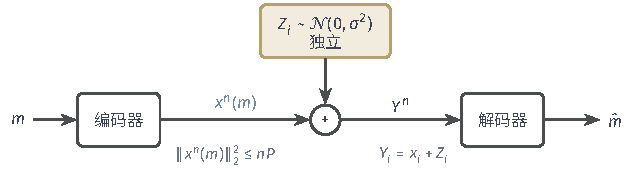
\includegraphics[width=107mm]{figures/07-probability/06-channel-coding/tikz/gcc-channel-model/figure.pdf}
 \caption{高斯信道上的块传输。编码器把消息$m$映成实数码字$x^n(m)$（蓝），它的能量不超过$nP$；每个坐标加上独立的噪声$Z_i\sim\mathcal{N}(0,\sigma^2)$（黄框），解码器根据输出块$Y^n$判决$\hat{m}$。}
 \label{fig:gcc-channel-model}
\end{BookInlineFigure}

\paragraph{不限制幅值时}
先看单次使用、只发两种消息的情形。发送$+A$或$-A$，接收端看输出的符号：输出为正判为$+A$，否则判为$-A$。发送$+A$而判错，需要噪声小于$-A$，概率是
\[
 \mathbb{P}(Z<-A)=\Phi\Bigl(-\frac{A}{\sigma}\Bigr) ,
\]
其中$\Phi$是标准高斯分布函数。取$\sigma=1$，$A=1$时这个概率是$0.159$，$A=3$时降到$0.00135$。图~\ref{fig:gcc-two-point}画出两种情形下的两条输出密度：幅值越大，两条钟形分得越开，重叠的尾部越小。

\begin{BookInlineFigure}
 \centering
 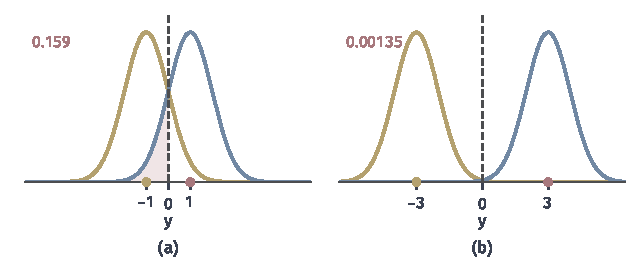
\includegraphics[width=108mm]{figures/07-probability/06-channel-coding/matplotlib/gcc-two-point/figure.pdf}
 \caption{两点输入$\pm A$经过$\sigma^2=1$的高斯噪声。黄线是发送$-A$时的输出密度，蓝线是发送$+A$时的输出密度，虚线是判决门限$0$，红色阴影是发送$+A$而判错的概率。(a)$A=1$，错误概率$0.159$。(b)$A=3$，错误概率$0.00135$。}
 \label{fig:gcc-two-point}
\end{BookInlineFigure}

幅值不受限制时，可靠传输没有上限。把间距固定为$d$，在实轴上放$K$个等距的输入点，每个点被判错的概率不超过$2\Phi(-d/(2\sigma))$，只要$d$足够大，这个概率可以任意小，而$K$可以任意大。于是每次使用可以近乎无错地送出$\log_2K$比特，$K$没有上界。同理，若$\sigma^2=0$，任意两个不同的实数都能被区分，一次使用就能送出任意多的比特。所以有意义的问题必须同时有两个前提：噪声方差为正，输入的幅值受到预算约束。

\paragraph{功率约束下的块码}
实际的发射设备受能量或平均功率的限制。约束加在每一条码字上：

\begin{definition}[功率约束下的块码]
\label{def:gcc-code}
设$P\geq0$。高斯信道上满足\term{功率约束}（power constraint）$P$的$(M,n)$码由编码器$f:\{1,\dots,M\}\to\mathbb{R}^n$与可测的解码器$g:\mathbb{R}^n\to\{1,\dots,M\}$组成，码字$x^n(m)=f(m)$对每条消息都满足
\begin{equation}
 \lVert x^n(m)\rVert_2^2=\sum_{i=1}^{n}x_i(m)^2\leq nP,\qquad m=1,\dots,M .
 \label{eq:gcc-power}
\end{equation}
\end{definition}

码率、条件错误概率、平均错误概率、最大错误概率和可达速率都沿用第~\ref{chap:discrete-channel-capacity}章的定义，只是把对输出块的求和换成对条件密度~\eqref{eq:gcc-block-density}的积分：
\begin{equation}
 \lambda_m=\int_{\{y^n:\,g(y^n)\neq m\}}p\bigl(y^n\mid x^n(m)\bigr)\,\mathrm{d}y^n ,
 \qquad P_{\mathrm{e}}=\frac1M\sum_{m=1}^{M}\lambda_m .
 \label{eq:gcc-errors}
\end{equation}
称$R$为功率$P$下的可达速率，若存在一列满足功率约束$P$的$(M_n,n)$码，$M_n\geq2^{nR}$且$P_{\mathrm{e}}\to0$。可达速率的上确界记作$C_{\mathrm{op}}(P)$。本章用$P$表示功率；分布写作带下标的$P_X$，概率写作$\mathbb{P}$，平均错误概率写作$P_{\mathrm{e}}$，三者不会混淆。

约束~\eqref{eq:gcc-power}有三点需要读清。

第一，它是沿一条码字的时间平均：$\frac1n\sum_ix_i(m)^2\leq P$。同一条码字可以在某些位置用大幅值、在另一些位置用小幅值，只要总能量不超预算。

第二，它对每一条码字分别成立，不允许一条码字超支、由另一条码字的节省来补偿。若只要求$\frac1M\sum_m\lVert x^n(m)\rVert_2^2\leq nP$，约束就变弱了。第~\ref{sec:gcc-coding}小节的逆定理说明，即使在这种较弱的约束下，速率也不能超过同一个上限。

第三，它是第~\ref{chap:discrete-channel-capacity}章输入成本约束的连续类比：成本函数取$c(x)=x^2$，预算取$\Gamma=P$。不同的是输入字母表不再有限，那里依赖有限单纯形紧性的论证都要重做。

$P=0$时，每条码字只能是零向量，不同消息的码字相同，只有$M=1$的码能做到无错，所以$C_{\mathrm{op}}(0)=0$。下文讨论容量公式时通常假设$P>0$，并在结论中注明端点。

\paragraph{噪声向量的长度}
把整块输出看成$\mathbb{R}^n$中的一个点，可以得到一幅几何图景。先看噪声向量$Z^n$的长度。由于$Z_i^2$独立同分布，期望为$\sigma^2$，第~\ref{chap:laws-of-large-numbers}章的弱大数律给出
\[
 \frac1n\lVert Z^n\rVert_2^2=\frac1n\sum_{i=1}^{n}Z_i^2\xrightarrow{\mathbb{P}}\sigma^2 .
\]
也就是说，块长很大时噪声向量的长度几乎总接近$\sqrt{n\sigma^2}$：$n$维高斯噪声集中在一个薄球壳上，而不是均匀地填满一个球。

图~\ref{fig:gcc-noise-norm}画出$\sigma^2=1$时$\lVert Z^n\rVert_2^2/n$的精确密度，它是$\chi^2_n$分布除以$n$。$\lVert Z^n\rVert_2^2/n$落在$[0.8,1.2]$中的概率，$n=4$时是$0.217$，$n=32$时是$0.579$，$n=256$时是$0.976$。

\begin{BookInlineFigure}
 \centering
 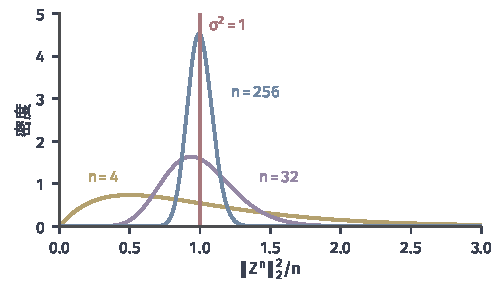
\includegraphics[width=84mm]{figures/07-probability/06-channel-coding/matplotlib/gcc-noise-norm/figure.pdf}
 \caption{$\sigma^2=1$时噪声向量的平均平方长度$\lVert Z^n\rVert_2^2/n$的密度，即$\chi^2_n/n$。黄、紫、蓝三条曲线分别对应$n=4,32,256$，红线是$\sigma^2=1$。块长越大，长度越集中在$\sqrt{n\sigma^2}$附近。}
 \label{fig:gcc-noise-norm}
\end{BookInlineFigure}

输出向量也有同样的现象。设码字满足$\lVert x^n\rVert_2^2\approx nP$，则
\[
 \frac1n\lVert x^n+Z^n\rVert_2^2=\frac1n\lVert x^n\rVert_2^2+\frac2n\langle x^n,Z^n\rangle+\frac1n\lVert Z^n\rVert_2^2 .
\]
中间的交叉项均值为零，方差为$4\sigma^2\lVert x^n\rVert_2^2/n^2\leq4\sigma^2P/n$，随$n$增大而趋于零；最后一项趋于$\sigma^2$。所以输出几乎总落在半径约$\sqrt{n(P+\sigma^2)}$的球内。

\paragraph{球的计数}
现在可以粗略地数一数能区分多少条消息。每条码字的输出集中在以码字为中心、半径约$\sqrt{n\sigma^2}$的小球附近；所有输出都在半径约$\sqrt{n(P+\sigma^2)}$的大球内。要从输出唯一认出码字，各个小球应当基本不重叠，于是码字数至多约为两球体积之比：
\[
 \frac{\bigl(\sqrt{n(P+\sigma^2)}\bigr)^{n}}{\bigl(\sqrt{n\sigma^2}\bigr)^{n}}
 =\Bigl(1+\frac{P}{\sigma^2}\Bigr)^{n/2} .
\]
这里用到了$n$维球的体积与半径的$n$次方成正比，比例常数在两球之间消去。取以2为底的对数再除以$n$，每次使用至多约送出
\[
 \frac12\log_2\Bigl(1+\frac{P}{\sigma^2}\Bigr)\ \text{比特}.
\]

全章的标量例子取$\sigma^2=1$，$P=3$。两球半径之比是$\sqrt{4}=2$，$n$维体积之比是$2^n$，每次使用约$1$比特。图~\ref{fig:gcc-sphere-packing}在平面上画出这幅图景；为了画得下，图中取$P/\sigma^2=8$。

\begin{BookInlineFigure}
 \centering
 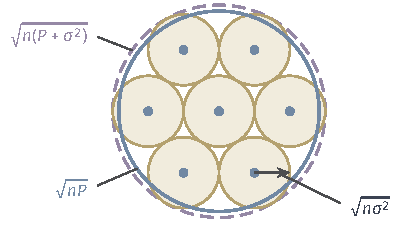
\includegraphics[width=68mm]{figures/07-probability/06-channel-coding/tikz/gcc-sphere-packing/figure.pdf}
 \caption{球的计数在平面上的示意（$n=2$，$P/\sigma^2=8$）。蓝点是码字，位于半径$\sqrt{nP}$的蓝色圆内；黄色小圆是半径$\sqrt{n\sigma^2}$的噪声球；所有输出落在半径$\sqrt{n(P+\sigma^2)}$的紫色虚线圆内。两圆面积之比是$9$，图中放下了$7$个互不重叠的噪声球。}
 \label{fig:gcc-sphere-packing}
\end{BookInlineFigure}

这个计数是启发，不是证明。体积之比只给出码字数的上限的猜测：它没有说明小球能否真的几乎不重叠地排满大球，也没有处理输出落在小球之外的情形。平面上的排列已经显示圆不能恰好铺满，图中$7$个小球只占大圆面积的$7/9$。下一节不再直接排列小球，而是先在单次使用上求互信息的最大值，再用随机选取的码字证明这个值可达；结果与上面的猜测一致。


\section{标量容量}
\label{sec:gcc-scalar}

球的计数猜出了$\frac12\log_2(1+P/\sigma^2)$。仿照第~\ref{chap:discrete-channel-capacity}章，严格的做法分两步：先把单次使用的输入看成随机变量$X$，在功率预算$\mathbb{E}[X^2]\leq P$下最大化互信息$I(X;Y)$；再证明这个最大值恰好是满足约束~\eqref{eq:gcc-power}的块码所能达到的速率极限。

\paragraph{单次使用的优化问题}
设$X$与$Z\sim\mathcal{N}(0,\sigma^2)$独立，$Y=X+Z$。输入不再限于有限个值，它可以是离散的、有密度的或两者混合的任意实值随机变量。互信息按第~\ref{chap:information-measures}章的一般定义理解为联合分布相对于边缘乘积的KL散度，
\[
 I(X;Y)=D_{\mathrm{KL}}\bigl(P_{XY}\,\Vert\,P_X\otimes P_Y\bigr),
\]
本章以比特计，即对数取以2为底。单次使用的优化问题是
\begin{equation}
 C(P)=\sup\bigl\{I(X;Y):\ X\text{与}Z\text{独立},\ \mathbb{E}[X^2]\leq P\bigr\} ,
 \label{eq:gcc-info-capacity}
\end{equation}
称为功率$P$下的信息容量。可行的输入分布组成一个无穷维的集合，这里先写上确界；下面会看到它能被取到。

\subsection{容量上界}
\label{sec:gcc-upper}

上界来自两个事实：输出$Y$的方差受预算控制；方差固定时，高斯分布的微分熵最大。后一个事实在第~\ref{chap:rate-distortion}章研究高斯信源时已经证明，这里重述结论，并回顾它的来源。

\begin{lemma}[固定方差的熵上界]
\label{lem:gcc-max-entropy}
设实值随机变量$Y$有密度$f$，方差$s\in(0,\infty)$，并且微分熵$h(Y)=-\int f\log_2f$有定义且有限。则
\begin{equation}
 h(Y)\leq\frac12\log_2(2\pi\mathrm{e}\,s),
 \label{eq:gcc-max-entropy}
\end{equation}
等号当且仅当$Y$服从高斯分布时成立。
\end{lemma}

回顾其理由：取与$Y$同均值$\mu$、同方差$s$的高斯密度$q$。$-\log_2q(y)$是$(y-\mu)^2$的一次函数，它在$Y$下的期望只依赖均值和方差，等于$\frac12\log_2(2\pi\mathrm{e}s)$。于是
\[
 0\leq D_{\mathrm{KL}}(f\Vert q)=-h(Y)+\frac12\log_2(2\pi\mathrm{e}\,s),
\]
等号当且仅当$f=q$几乎处处成立。高斯分布本身的微分熵正是右端，所以$h(Z)=\frac12\log_2(2\pi\mathrm{e}\sigma^2)$。

要把引理用在输出$Y$上，先要确认$Y$有密度、熵有限，并且互信息可以写成两个微分熵之差。这些都由“输入二阶矩有限、噪声是独立的高斯变量”保证。

\begin{lemma}[输出的密度与互信息]
\label{lem:gcc-output}
设$\mathbb{E}[X^2]<\infty$，$Z\sim\mathcal{N}(0,\sigma^2)$与$X$独立，$Y=X+Z$。则
\begin{enumerate}
 \item $Y$有密度$f_Y(y)=\mathbb{E}\bigl[g_{\sigma^2}(y-X)\bigr]$，并且$0<f_Y(y)\leq(2\pi\sigma^2)^{-1/2}$；
 \item $\mathbb{E}[Y^2]=\mathbb{E}[X^2]+\sigma^2$，并且$Y$的方差等于$X$的方差加上$\sigma^2$；
 \item $h(Y)$有限，并且
 \begin{equation}
  I(X;Y)=h(Y)-h(Z)=h(Y)-\frac12\log_2(2\pi\mathrm{e}\sigma^2) .
  \label{eq:gcc-mi-entropy}
 \end{equation}
\end{enumerate}
\end{lemma}

\begin{proof}
第一条。由独立性和Fubini定理，对任意$t$，
\[
 \mathbb{P}(Y\leq t)=\mathbb{E}\Bigl[\int_{-\infty}^{t}g_{\sigma^2}(y-X)\,\mathrm{d}y\Bigr]
 =\int_{-\infty}^{t}\mathbb{E}\bigl[g_{\sigma^2}(y-X)\bigr]\,\mathrm{d}y ,
\]
所以$f_Y(y)=\mathbb{E}[g_{\sigma^2}(y-X)]$是$Y$的密度。被平均的函数取值在$(0,(2\pi\sigma^2)^{-1/2}]$中，平均值也在这个范围内。

第二条。$X$与$Z$独立且$\mathbb{E}[Z]=0$，所以$\mathbb{E}[XZ]=0$，展开$(X+Z)^2$取期望即得前一式；独立变量的方差可加，即得后一式。

第三条。先说明$\log_2f_Y(Y)$可积。上界由第一条给出：$\log_2f_Y(y)\leq-\frac12\log_2(2\pi\sigma^2)$。下界用Jensen不等式：$\ln$是凹函数，
\[
 \begin{aligned}
  \ln f_Y(y)&=\ln\mathbb{E}\bigl[g_{\sigma^2}(y-X)\bigr]\geq\mathbb{E}\bigl[\ln g_{\sigma^2}(y-X)\bigr]\\
  &=-\frac12\ln(2\pi\sigma^2)-\frac{\mathbb{E}[(y-X)^2]}{2\sigma^2} .
 \end{aligned}
\]
再用$(y-x)^2\leq2y^2+2x^2$，得到
\[
 \ln f_Y(y)\geq-\frac12\ln(2\pi\sigma^2)-\frac{y^2+\mathbb{E}[X^2]}{\sigma^2} .
\]
两边夹住，$\lvert\ln f_Y(Y)\rvert$不超过常数加$Y^2/\sigma^2$，而$\mathbb{E}[Y^2]<\infty$，所以$h(Y)=-\mathbb{E}[\log_2f_Y(Y)]$有限。

再看互信息。对可测集$A,B$，由独立性，
\[
 \begin{aligned}
  P_{XY}(A\times B)&=\mathbb{E}\Bigl[\mathbf{1}_{A}(X)\int_Bg_{\sigma^2}(y-X)\,\mathrm{d}y\Bigr]\\
  &=\iint_{A\times B}\frac{g_{\sigma^2}(y-x)}{f_Y(y)}\,P_X(\mathrm{d}x)\,f_Y(y)\,\mathrm{d}y .
 \end{aligned}
\]
所以$r(x,y)=g_{\sigma^2}(y-x)/f_Y(y)$是$P_{XY}$相对于$P_X\otimes P_Y$的密度。KL散度是$\log_2r$在$P_{XY}$下的期望；在$(X,Y)$处$y-x=Z$，于是
\[
 I(X;Y)=\mathbb{E}\bigl[\log_2g_{\sigma^2}(Z)\bigr]-\mathbb{E}\bigl[\log_2f_Y(Y)\bigr]=-h(Z)+h(Y) .
\]
两个期望都有限，拆开是合法的。
\end{proof}

证明中密度$r$的存在性用的是卷四的Radon–Nikodym框架，可参考\BookChapterRef{chap:measure-densities}{卷四第8章“测度的密度”}。式~\eqref{eq:gcc-mi-entropy}的读法与离散情形相同：$h(Y)$度量输出的总分散程度，$h(Z)$是知道输入以后仍然剩下的分散程度，两者之差是观测输出对输入不确定性的减少。噪声加在输入之上、与输入独立，所以“知道输入后剩下的分散”总是同一个$h(Z)$，与输入怎样分布无关。

微分熵本身可以为负，单独一项没有“需要多少比特”的含义。例如$\sigma^2=0.01$时，
\[
 h(Z)=\frac12\log_2(2\pi\mathrm{e}\cdot0.01)=-1.27\ \text{比特}.
\]
这不妨碍式~\eqref{eq:gcc-mi-entropy}：把输入、输出同时乘以常数$a\neq0$，$h(Y)$和$h(Z)$都增加$\log_2\lvert a\rvert$，差不变，与互信息在可逆变换下不变一致。引理的第三条之所以要先证明$h(Y)$有限，正是为了保证这个差不是“无穷减无穷”。

\begin{theorem}[互信息的上界]
\label{thm:gcc-upper}
设$Z\sim\mathcal{N}(0,\sigma^2)$，$\sigma^2>0$，$X$与$Z$独立且$\mathbb{E}[X^2]\leq P$。则
\begin{equation}
 I(X;X+Z)\leq\frac12\log_2\Bigl(1+\frac{P}{\sigma^2}\Bigr) .
 \label{eq:gcc-upper}
\end{equation}
\end{theorem}

\begin{proof}
由引理~\ref{lem:gcc-output}，$Y=X+Z$有密度，$h(Y)$有限，方差满足
\[
 \sigma^2\leq\operatorname{Var}(Y)\leq\mathbb{E}[Y^2]=\mathbb{E}[X^2]+\sigma^2\leq P+\sigma^2 .
\]
方差为正且有限，引理~\ref{lem:gcc-max-entropy}适用，再利用$\log_2$单调递增，得到
\[
 h(Y)\leq\frac12\log_2\bigl(2\pi\mathrm{e}\operatorname{Var}(Y)\bigr)\leq\frac12\log_2\bigl(2\pi\mathrm{e}(P+\sigma^2)\bigr) .
\]
代入式~\eqref{eq:gcc-mi-entropy}，两项中的$2\pi\mathrm{e}$相消，
\[
 I(X;Y)\leq\frac12\log_2\bigl(2\pi\mathrm{e}(P+\sigma^2)\bigr)-\frac12\log_2(2\pi\mathrm{e}\sigma^2)=\frac12\log_2\frac{P+\sigma^2}{\sigma^2} .
\]
\end{proof}

定理的三个条件各有作用。$\sigma^2>0$保证$Y$有密度、$h(Z)$有限；若$\sigma^2=0$，$h(Z)$不存在，而上一节已经看到容量没有上限。$X$与$Z$独立保证知道输入后剩下的熵恰好是$h(Z)$，也保证方差相加。$\mathbb{E}[X^2]\leq P$只控制二阶矩，它同时约束了均值和方差。二阶矩等于均值的平方加方差，而输出熵只依赖于$Y$的分布形状和分散程度，平移不改变微分熵；所以均值非零的输入不带来任何好处，只是把一部分预算花在了平移上。

\paragraph{例：同一预算下的三种输入}
取$\sigma^2=1$，$P=3$。噪声的熵是$h(Z)=\frac12\log_2(2\pi\mathrm{e})=2.047$比特，输出熵的上界是$\frac12\log_2(8\pi\mathrm{e})=3.047$比特，所以任何满足预算的输入都有$I(X;Y)\leq1$比特。

比较三种功率都等于$3$的输入：等概率取$\pm\sqrt3$的二点输入，$[-3,3]$上的均匀输入，以及$\mathcal{N}(0,3)$。数值积分给出
\[
 I_{\text{二点}}=0.845,\qquad I_{\text{均匀}}=0.972,\qquad I_{\text{高斯}}=1.000 .
\]
图~\ref{fig:gcc-output-entropy}画出三种输入对应的输出密度。三者方差相同，二点输入的输出是两个钟形的叠加，中间凹下；均匀输入的输出顶部较平；只有高斯输入的输出仍是高斯形状。方差相同时形状越接近高斯，输出熵越大，互信息也越大。

\begin{BookInlineFigure}
 \centering
 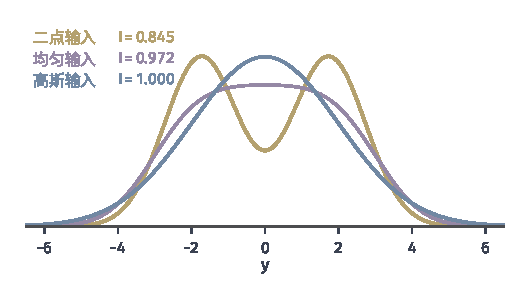
\includegraphics[width=88mm]{figures/07-probability/06-channel-coding/matplotlib/gcc-output-entropy/figure.pdf}
 \caption{$\sigma^2=1$时，三种功率都为$3$的输入经过信道后的输出密度：二点输入$\pm\sqrt3$（黄），$[-3,3]$上的均匀输入（紫），$\mathcal{N}(0,3)$（蓝）。三条输出的方差都是$4$，图中给出对应的互信息（比特）。}
 \label{fig:gcc-output-entropy}
\end{BookInlineFigure}

\subsection{最优输入}
\label{sec:gcc-optimal-input}

上界~\eqref{eq:gcc-upper}的证明中有两处放大：$\operatorname{Var}(Y)\leq P+\sigma^2$，以及固定方差的熵上界。要使两处都取等号，输出必须是方差恰为$P+\sigma^2$的高斯变量。独立高斯变量之和仍是高斯变量（第~\ref{chap:random-variable-transformations}章），所以取$X\sim\mathcal{N}(0,P)$即可：此时$Y\sim\mathcal{N}(0,P+\sigma^2)$。

\begin{theorem}[高斯信道的信息容量]
\label{thm:gcc-capacity}
设$\sigma^2>0$，$P\geq0$。式~\eqref{eq:gcc-info-capacity}中的上确界可以取到，并且
\begin{equation}
 C(P)=\frac12\log_2\Bigl(1+\frac{P}{\sigma^2}\Bigr)\quad\text{比特每次信道使用}.
 \label{eq:gcc-capacity}
\end{equation}
达到最大值的输入分布唯一，是$\mathcal{N}(0,P)$（$P=0$时理解为恒等于零的输入）。
\end{theorem}

\begin{proof}
上界由定理~\ref{thm:gcc-upper}给出。$P>0$时取$X\sim\mathcal{N}(0,P)$与$Z$独立，$Y\sim\mathcal{N}(0,P+\sigma^2)$，由式~\eqref{eq:gcc-mi-entropy}，
\[
 I(X;Y)=\frac12\log_2\bigl(2\pi\mathrm{e}(P+\sigma^2)\bigr)-\frac12\log_2(2\pi\mathrm{e}\sigma^2)=C(P) .
\]
$P=0$时只能$X=0$，$Y=Z$，互信息为零，与公式一致。

再证唯一性，设$P>0$且某个可行输入$X$达到$C(P)$。上界证明中的两处不等式都必须取等号：$Y$的方差等于$P+\sigma^2$，且$Y$是高斯变量。$Y$的方差是$X$的方差加$\sigma^2$，所以
\[
 \operatorname{Var}(X)=P\geq\mathbb{E}[X^2]=(\mathbb{E}X)^2+\operatorname{Var}(X),
\]
于是$\mathbb{E}[X]=0$，$Y\sim\mathcal{N}(0,P+\sigma^2)$。用第~\ref{chap:weak-convergence-of-distributions}章的特征函数，独立和的特征函数是乘积：
\[
 \mathrm{e}^{-(P+\sigma^2)t^2/2}=\phi_Y(t)=\phi_X(t)\,\phi_Z(t)=\phi_X(t)\,\mathrm{e}^{-\sigma^2t^2/2} .
\]
$\phi_Z(t)$处处不为零，两边相除得$\phi_X(t)=\mathrm{e}^{-Pt^2/2}$。特征函数唯一确定分布，所以$X\sim\mathcal{N}(0,P)$。
\end{proof}

比值$P/\sigma^2$称为\term{信噪比}（signal-to-noise ratio，SNR）。容量只依赖信噪比：把输出除以$\sigma$得到噪声方差为$1$、功率为$P/\sigma^2$的信道，接收端可以随时这样做或撤销，传输能力不变。工程上常用分贝表示信噪比，即$10\log_{10}(P/\sigma^2)$。

\paragraph{读容量公式}
公式~\eqref{eq:gcc-capacity}的单位是比特每次实值信道使用。全章的例子$P/\sigma^2=3$给出
\[
 C=\tfrac12\log_2 4=1\ \text{比特每次},
\]
与球的计数一致。把信噪比提到$15$，$1+P/\sigma^2$从$4$变成$16$，容量变成$2$比特：功率增加到五倍，容量只增加一倍。

容量是信噪比的凹函数，图~\ref{fig:gcc-capacity-curve}分两段读它。信噪比很小时，由$\ln(1+u)\leq u$且$u\to0$时二者之比趋于$1$，
\[
 C(P)\leq\frac{\log_2\mathrm{e}}{2}\cdot\frac{P}{\sigma^2},\qquad
 \frac{C(P)}{P/\sigma^2}\to\frac{\log_2\mathrm{e}}{2}\approx0.721\quad(P\to0) .
\]
低信噪比时容量与功率近似成正比，每单位信噪比约值$0.721$比特。信噪比很大时，$\log_2(1+u)-\log_2u\to0$，容量接近$\frac12\log_2(P/\sigma^2)$，功率每增加到四倍（约$6.02$分贝），容量只多$1$比特。

\begin{BookInlineFigure}
 \centering
 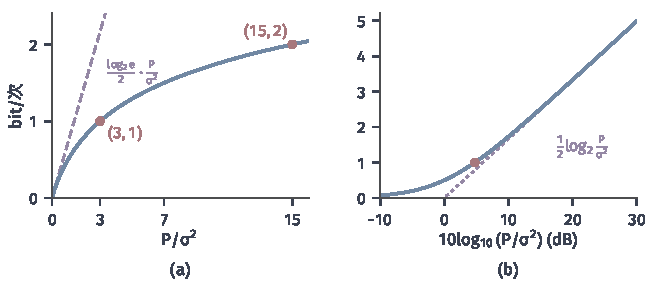
\includegraphics[width=110mm]{figures/07-probability/06-channel-coding/matplotlib/gcc-capacity-curve/figure.pdf}
 \caption{标量高斯信道的容量$C=\frac12\log_2(1+P/\sigma^2)$（蓝）。(a)线性横轴，红点是$(3,1)$和$(15,2)$，紫色虚线是低信噪比时的切线$\frac{\log_2\mathrm{e}}{2}\cdot\frac{P}{\sigma^2}$。(b)横轴为分贝，紫色点线是高信噪比的渐近线$\frac12\log_2(P/\sigma^2)$，斜率约为每$6.02$分贝$1$比特。}
 \label{fig:gcc-capacity-curve}
\end{BookInlineFigure}

\paragraph{有限个输入值的代价}
高斯输入要用到所有实数幅值。若只允许有限个输入值，互信息会低于$C(P)$。等概率二点输入$\pm\sqrt{P}$的互信息不超过$1$比特，无论功率多大；若接收端只记录输出的正负号，信道变成翻转概率$p=\Phi(-\sqrt{P/\sigma^2})$的二元对称信道，速率降为第~\ref{chap:discrete-channel-capacity}章的$1-h_2(p)$，$h_2$是以比特计的二元熵函数。$P/\sigma^2=3$时，$p=0.0416$，三个数是
\[
 C=1.000,\qquad I_{\text{二点}}=0.845,\qquad 1-h_2(p)=0.750 .
\]

图~\ref{fig:gcc-binary-input}把三条曲线画在一起。低信噪比时三者差距很小，因为容量本来就远小于$1$比特，二点输入已经够用；信噪比升高后，二点输入的曲线停在$1$比特，高斯输入继续增长。符号判决丢掉了输出幅值中的可信度信息，由第~\ref{chap:information-measures}章的数据处理不等式，它只能减少互信息。

\begin{BookInlineFigure}
 \centering
 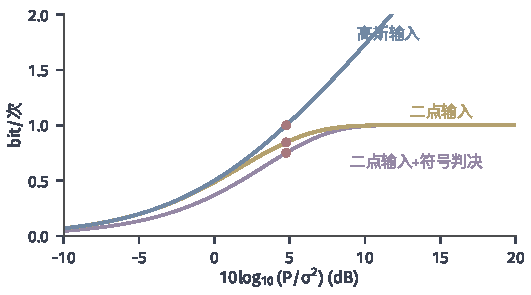
\includegraphics[width=90mm]{figures/07-probability/06-channel-coding/matplotlib/gcc-binary-input/figure.pdf}
 \caption{$\sigma^2=1$时三种传输方式的速率随信噪比（分贝）的变化。蓝：高斯输入，即容量；黄：等概率二点输入，接收端使用实数输出；紫：同样的二点输入，接收端只取输出的正负号。红点对应$P/\sigma^2=3$。}
 \label{fig:gcc-binary-input}
\end{BookInlineFigure}

\paragraph{计量单位}
$C(P)$是每次实值使用的比特数，功率$P$是每次使用的平均能量。改变计量方式时，两者要一起换算。

若每个时刻传送的是一个复数，可以把实部和虚部看成两次实值使用。常见的约定是复噪声的实部与虚部独立，各有方差$\sigma^2/2$，复输入满足$\mathbb{E}\lvert X\rvert^2\leq P$。实部和虚部各分到功率$P/2$时，两次实值使用合计
\[
 2\cdot\frac12\log_2\Bigl(1+\frac{P/2}{\sigma^2/2}\Bigr)=\log_2\Bigl(1+\frac{P}{\sigma^2}\Bigr)\ \text{比特每次复值使用}.
\]
平均分配为什么最优，由第~\ref{sec:gcc-parallel}节的平行信道回答。

若信道每秒使用$m$次，每秒能可靠传送$m\,C(P)$比特，前提是这$m$次使用仍满足本章的模型：噪声独立、方差都是$\sigma^2$，并且$P$指每次使用的功率。若改为给定每秒的总能量，或使用频率改变时噪声方差也随之改变，就要先把这些量折算回每次使用，再代入公式~\eqref{eq:gcc-capacity}。

\subsection{满足功率约束的编码}
\label{sec:gcc-coding}

信息容量是单次使用上的优化值。它是否就是块码的速率极限$C_{\mathrm{op}}(P)$，需要两个方向的证明：低于$C(P)$的速率都可达，高于$C(P)$的速率都不可达。

\begin{theorem}[高斯信道的编码定理]
\label{thm:gcc-coding}
设$\sigma^2>0$，$P>0$。
\begin{enumerate}
 \item 对每个$R<C(P)$，存在一列满足功率约束$P$的$(M_n,n)$码，$M_n\geq2^{nR}$，并且最大错误概率$\lambda_{\max}\to0$。
 \item 任意一列满足功率约束$P$的码，若平均错误概率$P_{\mathrm{e}}\to0$，则$\limsup_{n\to\infty}\frac1n\log_2M_n\leq C(P)$。
\end{enumerate}
因此$C_{\mathrm{op}}(P)=C(P)$；$P=0$时两者都是$0$。
\end{theorem}

\paragraph{为什么不能照搬典型集计数}
第~\ref{chap:discrete-channel-capacity}章的可达性证明数的是典型序列的个数：有限字母表上长为$n$的序列只有有限多个，每个典型序列的概率约为$2^{-nH}$。连续输入下，任何一个具体序列的概率都是零，“个数”没有意义，也不能把$2^{-nH}$中的$H$直接换成可以为负的微分熵。可以保留的是另一样东西：信道条件密度与输出边缘密度之比。下面用它的对数代替典型性。

\paragraph{信息密度}
选一个略低于预算的功率$P'\in(0,P)$，让码字的坐标独立地服从$\mathcal{N}(0,P')$。在这个输入分布下，输出的边缘密度是$g_{P'+\sigma^2}$。

\begin{definition}[信息密度]
\label{def:gcc-info-density}
对输入分布$\mathcal{N}(0,P')$，单次使用的\term{信息密度}（information density）是
\begin{equation}
 i(x;y)=\log_2\frac{g_{\sigma^2}(y-x)}{g_{P'+\sigma^2}(y)} ,
 \label{eq:gcc-info-density}
\end{equation}
长度为$n$的块上的信息密度是逐坐标之和$i_n(x^n;y^n)=\sum_{i=1}^{n}i(x_i;y_i)$。
\end{definition}

$i(x;y)$比较两种解释：$y$是$x$经过噪声得到的，还是与$x$无关地随机出现的。它为正，说明$y$更像由$x$产生。把两个高斯密度代入并展开，
\begin{equation}
 i(x;y)=C(P')+\frac{\log_2\mathrm{e}}{2}\Bigl(\frac{y^2}{P'+\sigma^2}-\frac{(y-x)^2}{\sigma^2}\Bigr) .
 \label{eq:gcc-info-density-explicit}
\end{equation}
信息密度有两个用途，分别对应发送的码字和其余的码字。

第一，对发送的码字及其输出，$i_n$集中在$nC(P')$附近。设$X\sim\mathcal{N}(0,P')$，$Y=X+Z$。此时$Y^2/(P'+\sigma^2)$与$Z^2/\sigma^2$都服从$\chi^2_1$，均值为$1$，所以$\mathbb{E}[i(X;Y)]=C(P')$，这正是式~\eqref{eq:gcc-mi-entropy}的互信息。再算方差：两项的方差都是$2$；$Y$与$Z$是联合高斯的零均值变量，对这样的变量有
\[
 \operatorname{Cov}(Y^2,Z^2)=2\operatorname{Cov}(Y,Z)^2=2\sigma^4 ,
\]
因此
\[
 \operatorname{Var}\Bigl(\frac{Y^2}{P'+\sigma^2}-\frac{Z^2}{\sigma^2}\Bigr)=2+2-\frac{4\sigma^4}{(P'+\sigma^2)\sigma^2}=\frac{4P'}{P'+\sigma^2} .
\]
乘以$(\log_2\mathrm{e}/2)^2$，单次信息密度的方差是
\begin{equation}
 V(P')=\operatorname{Var}\bigl(i(X;Y)\bigr)=(\log_2\mathrm{e})^2\,\frac{P'}{P'+\sigma^2} .
 \label{eq:gcc-info-variance}
\end{equation}
$i_n$是$n$个独立同分布项之和，均值$nC(P')$，方差$nV(P')$。

第二，对与输出无关的码字，$i_n$很少超过高的门限。设$\bar{X}^n$的坐标独立服从$\mathcal{N}(0,P')$，与$Y^n$独立，$Y^n$的坐标独立服从$\mathcal{N}(0,P'+\sigma^2)$。$(\bar{X}^n,Y^n)$的联合密度是乘积$q(x^n,y^n)=f(x^n)\prod_ig_{P'+\sigma^2}(y_i)$，而发送与输出配对时的联合密度是$p(x^n,y^n)=f(x^n)\prod_ig_{\sigma^2}(y_i-x_i)$，$f$是输入块的密度。由定义，二者之比正是
\[
 \frac{q(x^n,y^n)}{p(x^n,y^n)}=2^{-i_n(x^n;y^n)} .
\]
于是对任意$\gamma$，
\begin{equation}
 \mathbb{P}\bigl(i_n(\bar{X}^n;Y^n)>n\gamma\bigr)=\int_{\{i_n>n\gamma\}}2^{-i_n}\,p\leq2^{-n\gamma}\int p=2^{-n\gamma} .
 \label{eq:gcc-change-of-measure}
\end{equation}
这一步把“独立配对”的概率换成“发送配对”的积分，换算因子就是$2^{-i_n}$，在门限以上它不超过$2^{-n\gamma}$。

\paragraph{例：信息密度的两种分布}
取$\sigma^2=1$，$P'=3$。发送配对时$\mathbb{E}[i]=C(3)=1$，$V=(\log_2\mathrm{e})^2\cdot\frac34=1.561$。独立配对时，$\mathbb{E}[(Y-\bar{X})^2]=(P'+\sigma^2)+P'=7$，代入式~\eqref{eq:gcc-info-density-explicit}，
\[
 \mathbb{E}[i(\bar{X};Y)]=1+\frac{\log_2\mathrm{e}}{2}\Bigl(1-7\Bigr)=1-3\log_2\mathrm{e}=-3.33 .
\]
图~\ref{fig:gcc-info-density}画出$n=20$与$n=200$时两种配对的$i_n/n$的直方图。块长增大，两个直方图分别收拢到$1$和$-3.33$；在两者之间放一个门限$\gamma$，发送的码字几乎总在门限之上，独立的码字几乎总在门限之下。

\begin{BookInlineFigure}
 \centering
 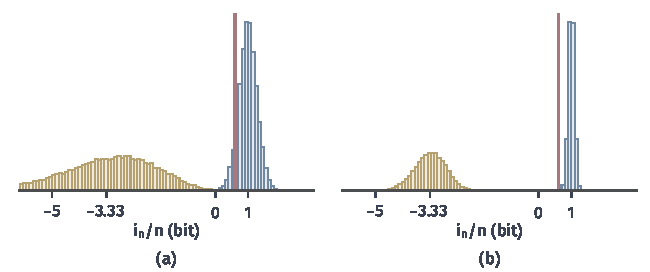
\includegraphics[width=110mm]{figures/07-probability/06-channel-coding/matplotlib/gcc-info-density/figure.pdf}
 \caption{$\sigma^2=1$、码字坐标服从$\mathcal{N}(0,3)$时归一化信息密度$i_n/n$的直方图（种子$7$，每个直方图$20000$对）。蓝：发送的码字与其输出，均值$1$；黄：与输出独立的码字，均值$-3.33$。红线是门限$\gamma=0.6$。(a)$n=20$，蓝色样本有$7.3\%$落在门限以下。(b)$n=200$，没有蓝色样本落在门限以下，也没有黄色样本落在门限以上。}
 \label{fig:gcc-info-density}
\end{BookInlineFigure}

\paragraph{随机码本与阈值判决}
现在构造码。给定$R<C(P)$，由$C$的连续性和严格单调性，可以依次选出
\[
 0<P'<P,\qquad R<\gamma<C(P') .
\]
取$M_n=2^{\lceil nR\rceil+1}$。码本由$M_n$个独立的随机码字$X^n(1),\dots,X^n(M_n)$组成，每个码字的坐标独立服从$\mathcal{N}(0,P')$。解码采用\term{阈值判决}（threshold decoding）：收到$y^n$后，若恰有一个$m$满足$i_n(X^n(m);y^n)>n\gamma$，判为这个$m$；否则判为$1$。

随机码字有可能超过预算，这样的码字不允许发送。分析时采取保守的记账：若$\lVert X^n(m)\rVert_2^2>nP$，就把消息$m$的条件错误概率记为$1$。

\paragraph{例：一次阈值判决}
用一个极小的码本走一遍判决过程。取$\sigma^2=1$，$P'=3$，$n=2$，门限$\gamma=0.6$，即要求$i_2>1.2$。三条码字和收到的输出是
\[
 \begin{gathered}
  x^2(1)=(1.5,-2.0),\quad x^2(2)=(-1.0,1.0),\quad x^2(3)=(2.0,1.5);\\
  y^2=(1.2,-1.4) .
 \end{gathered}
\]
由式~\eqref{eq:gcc-info-density-explicit}，此时
\[
 i(x;y)=1+\frac{\log_2\mathrm{e}}{2}\Bigl(\frac{y^2}{4}-(y-x)^2\Bigr) .
\]
对码字$1$的第一个坐标，$y^2/4=0.36$，$(y-x)^2=0.09$，代入得$1.195$；第二个坐标得$1.094$。三条码字的块信息密度分别是
\[
 i_2(x^2(1);y^2)=2.289,\quad i_2(x^2(2);y^2)=-5.033,\quad i_2(x^2(3);y^2)=-3.915 .
\]
只有码字$1$越过$1.2$，判为消息$1$。码字$3$的第一个坐标与输出也相当接近，信息密度为$0.798$，但第二个坐标相差$2.9$，在噪声标准差为$1$的信道上很不可能，贡献了$-4.713$，整块被否决。块信息密度把各坐标的证据加起来，一个坐标上的偶然吻合抵不过其他坐标上的明显不符。

\paragraph{三类错误}
由对称性，只需分析消息$1$，并对码本的随机性取平均。消息$1$被记为错误，只可能是下面三件事之一发生：
\begin{enumerate}
 \item $E_0$：码字超预算，$\lVert X^n(1)\rVert_2^2>nP$；
 \item $E_1$：发送的码字没有越过门限，$i_n(X^n(1);Y^n)\leq n\gamma$；
 \item $E_2$：某个其他码字越过了门限，即存在$m\neq1$使$i_n(X^n(m);Y^n)>n\gamma$。
\end{enumerate}
三件事都不发生时，恰有消息$1$越过门限，判决正确。三个概率可以分别估计。

$E_0$：$X_i^2$独立同分布，均值$P'$，方差$2P'^2$。由第~\ref{chap:tail-probabilities}章的Chebyshev不等式，
\[
 \mathbb{P}(E_0)=\mathbb{P}\Bigl(\sum_{i=1}^{n}(X_i^2-P')>n(P-P')\Bigr)\leq\frac{2P'^2}{n(P-P')^2} .
\]

$E_1$：$i_n$的均值是$nC(P')$，方差是$nV(P')$，门限$n\gamma$比均值低$n(C(P')-\gamma)$。同样由Chebyshev不等式，
\[
 \mathbb{P}(E_1)\leq\frac{V(P')}{n\bigl(C(P')-\gamma\bigr)^2} .
\]

$E_2$：每个$m\neq1$的码字与发送的码字独立，也与噪声独立，所以与$Y^n$独立，式~\eqref{eq:gcc-change-of-measure}适用。对$M_n-1$个码字用并集界，并利用$M_n\leq2^{nR+2}$，
\[
 \mathbb{P}(E_2)\leq(M_n-1)\,2^{-n\gamma}\leq4\cdot2^{-n(\gamma-R)} .
\]

三项相加，对码本取平均后，消息$1$的记账错误概率不超过
\begin{equation}
 \varepsilon_n=\frac{2P'^2}{n(P-P')^2}+\frac{V(P')}{n\bigl(C(P')-\gamma\bigr)^2}+4\cdot2^{-n(\gamma-R)} ,
 \label{eq:gcc-random-code-bound}
\end{equation}
三项都随$n\to\infty$趋于零。前两项来自大数律，按$1/n$减小；第三项来自门限与码率之间的余量$\gamma-R$，按指数减小。

以$\sigma^2=1$、$P=3$、$R=0.5$为例，取$P'=2.4$，$\gamma=0.7$。此时$C(P')=\frac12\log_2 3.4=0.883$，$V(P')=1.469$。$n=400$时式~\eqref{eq:gcc-random-code-bound}的三项约为
\[
 0.080,\qquad 0.110,\qquad 3\times10^{-24} .
\]
Chebyshev界相当粗：图~\ref{fig:gcc-codeword-energy}的精确计算表明，$n=400$时码字超预算的概率只有$0.00048$，而不是$0.080$。证明只需要这些界趋于零，不需要它们精确。

\begin{BookInlineFigure}
 \centering
 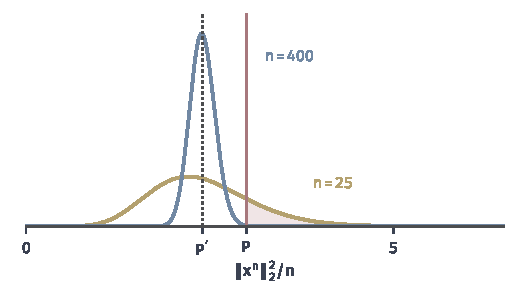
\includegraphics[width=88mm]{figures/07-probability/06-channel-coding/matplotlib/gcc-codeword-energy/figure.pdf}
 \caption{坐标独立服从$\mathcal{N}(0,P')$的随机码字的每坐标能量$\lVert x^n\rVert_2^2/n$的精确密度，$P'=2.4$，预算$P=3$（红线），点线标出$P'$。黄：$n=25$；蓝：$n=400$。红色阴影是超预算的概率，$n=25$时为$0.181$，$n=400$时为$0.00048$。}
 \label{fig:gcc-codeword-energy}
\end{BookInlineFigure}

\paragraph{从随机码本到确定的码}
式~\eqref{eq:gcc-random-code-bound}是对码本取平均的结果。由对称性，每条消息的平均记账错误都相同，所以$\frac1{M_n}\sum_m\tilde{\lambda}_m$对码本的平均也不超过$\varepsilon_n$，其中$\tilde{\lambda}_m$表示消息$m$的记账错误概率。平均值不超过$\varepsilon_n$，至少有一个码本取到不超过$\varepsilon_n$的值；固定这个码本。

这个码本中，记账错误超过$2\varepsilon_n$的消息至多占一半，否则平均值会超过$\varepsilon_n$。删去记账错误最大的一半消息，保留$M_n/2=2^{\lceil nR\rceil}\geq2^{nR}$条，每条都满足$\tilde{\lambda}_m\leq2\varepsilon_n$。当$n$足够大使$2\varepsilon_n<1$时，被保留的码字都不超预算，因为超预算的码字记账错误是$1$。

解码器改为只在保留的码字中做阈值判决。对一条保留的消息，新的错误事件包含在原来的$E_1$与“某个保留的其他码字越过门限”之并中，后者又包含在原来的$E_2$中，所以错误概率不会增加。这样得到的码满足功率约束，码率至少为$R$，最大错误概率不超过$2\varepsilon_n\to0$，定理~\ref{thm:gcc-coding}的第一条得证。

\begin{BookInlineFigure}
 \centering
 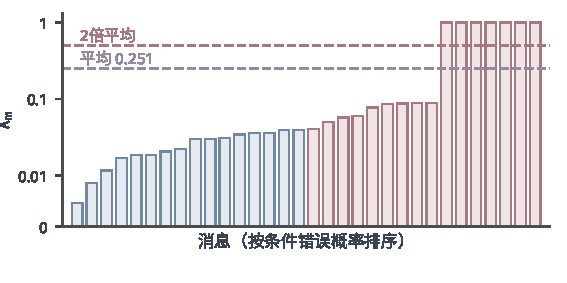
\includegraphics[width=96mm]{figures/07-probability/06-channel-coding/matplotlib/gcc-expurgation/figure.pdf}
 \caption{一个随机高斯码本（种子$5$，$n=12$，$M=32$，$P'=2.4$，$P=3$，$\sigma^2=1$，最近码字判决）中各消息的条件错误概率$\lambda_m$，按大小排序，每条消息用$20000$次噪声模拟估计。超预算的$7$个码字记为$1$。紫色虚线是平均值$0.251$，红色虚线是平均值的两倍；红色柱是删去的一半，保留的消息错误都在$0.04$以下。纵轴在$0.01$以下为线性刻度，以上为对数刻度。}
 \label{fig:gcc-expurgation}
\end{BookInlineFigure}

图~\ref{fig:gcc-expurgation}在一个很短的码上演示这一步。码长只有$12$时，$32$个随机码字中有$7$个超预算，把平均错误抬到$0.251$；删去最差的一半，超预算的码字全部被删掉，剩下的$16$条消息错误都在$0.04$以下。块长增大时，超预算的比例和其他错误都趋于零，删去一半只让码率损失$1/n$。

\paragraph{块长的作用}
证明保证错误趋于零，但没有说多长的块才够。图~\ref{fig:gcc-random-code}用模拟给出一个印象：码率固定为$R=\frac12$，码字取随机方向、长度恰为$\sqrt{nP}$，从而每条码字都恰好用满预算，接收端选与输出最近的码字。$C(P)=\frac12$对应$P/\sigma^2=1$，即$0$分贝。块长从$8$增加到$32$，错误率曲线变陡，在容量对应的信噪比右侧下降得越来越快；但$n=32$时，要把错误率压到$10^{-3}$，信噪比仍需高出约$4$分贝。逼近容量需要长得多的块和高效的译码方法，这是第~\ref{chap:channel-codes}章的话题。

\begin{BookInlineFigure}
 \centering
 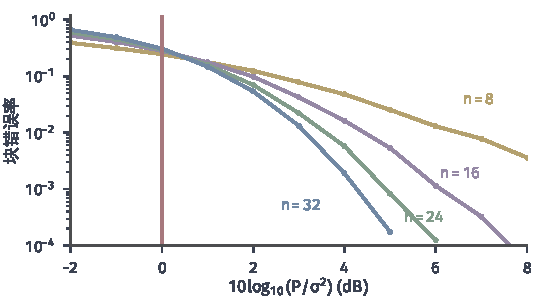
\includegraphics[width=92mm]{figures/07-probability/06-channel-coding/matplotlib/gcc-random-code/figure.pdf}
 \caption{码率$R=\frac12$的随机码在$\sigma^2=1$的高斯信道上的块错误率随信噪比（分贝）的变化，最近码字判决。码字是随机方向上长度为$\sqrt{nP}$的向量。黄、紫、绿、蓝分别对应$n=8,16,24,32$（$M=2^{n/2}$），每点模拟$40000$条消息（种子$11$）。红线是$C(P)=\frac12$对应的$0$分贝。}
 \label{fig:gcc-random-code}
\end{BookInlineFigure}

\paragraph{逆定理}
现在证明第二条：速率超过$C(P)$时，错误不能趋于零。思路与离散信道相同，只是单次互信息的上界换成定理~\ref{thm:gcc-upper}，并且要处理各时刻功率不同的情形。

设$(M,n)$码满足功率约束$P$，消息$W$在$\{1,\dots,M\}$上均匀分布，$X^n=x^n(W)$，$Y^n$是输出。第$i$个时刻在消息上的平均功率记作
\[
 P_i=\mathbb{E}[X_i^2]=\frac1M\sum_{m=1}^{M}x_i(m)^2 .
\]
对$i$求平均，由约束~\eqref{eq:gcc-power}，
\[
 \frac1n\sum_{i=1}^{n}P_i=\frac1M\sum_{m=1}^{M}\frac1n\lVert x^n(m)\rVert_2^2\leq P .
\]

第一步，由第~\ref{chap:information-measures}章的Fano不等式和数据处理不等式，
\[
 \log_2M=H(W)=I(W;Y^n)+H(W\mid Y^n)\leq I(X^n;Y^n)+1+P_{\mathrm{e}}\log_2M .
\]

第二步，上界$I(X^n;Y^n)$。$X^n$只取有限个值，引理~\ref{lem:gcc-output}的证明逐字推广到$n$维：$Y^n$有密度，$h(Y^n)$有限，并且$I(X^n;Y^n)=h(Y^n)-h(Z^n)$。噪声坐标独立，$h(Z^n)=\sum_ih(Z_i)$；由微分熵的链式法则和“条件化不增加熵”，$h(Y^n)\leq\sum_ih(Y_i)$。于是
\[
 I(X^n;Y^n)\leq\sum_{i=1}^{n}\bigl(h(Y_i)-h(Z_i)\bigr)\leq\sum_{i=1}^{n}C(P_i) ,
\]
最后一步对每个时刻用了定理~\ref{thm:gcc-upper}的证明：$\operatorname{Var}(Y_i)\leq P_i+\sigma^2$。

第三步，用凹性合并各时刻。$C(p)=\frac12\log_2(1+p/\sigma^2)$是$p$的凹增函数，由Jensen不等式，
\[
 \sum_{i=1}^{n}C(P_i)\leq n\,C\Bigl(\frac1n\sum_{i=1}^{n}P_i\Bigr)\leq n\,C(P) .
\]
图~\ref{fig:gcc-concavity}说明这一步：把功率在时刻之间不均匀地分配，各时刻上界的平均落在弦上，低于平均功率处的曲线值。

\begin{BookInlineFigure}
 \centering
 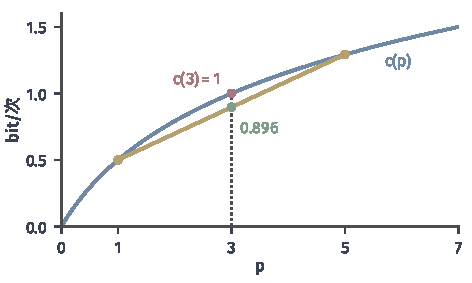
\includegraphics[width=80mm]{figures/07-probability/06-channel-coding/matplotlib/gcc-concavity/figure.pdf}
 \caption{$c(p)=\frac12\log_2(1+p)$（蓝，$\sigma^2=1$）的凹性。一半时刻用功率$1$、一半用$5$，平均功率为$3$；各时刻上界的平均是弦的中点$0.896$（绿），低于$c(3)=1$（红）。}
 \label{fig:gcc-concavity}
\end{BookInlineFigure}

三步合起来，
\begin{equation}
 \log_2M\leq\frac{n\,C(P)+1}{1-P_{\mathrm{e}}} .
 \label{eq:gcc-converse}
\end{equation}
对一列满足约束的码，若$P_{\mathrm{e}}\to0$，两边除以$n$再取上极限，便知码率$\frac1n\log_2M_n$的上极限不超过$C(P)$。定理~\ref{thm:gcc-coding}的第二条得证。

式~\eqref{eq:gcc-converse}也给出错误的下界。以$\sigma^2=1$、$P=3$为例，若码率为$1.2$比特，$\log_2M=1.2n$，整理得
\[
 P_{\mathrm{e}}\geq1-\frac{n+1}{1.2n}\to\frac16 .
\]
块再长，平均错误也不会低于约$16.7\%$。错误概率实际上趋于一，这称为强逆定理，它在这个模型中也成立，但证明需要对信息密度作更细的集中估计，本章不给出证明。

逆定理只用了$\frac1n\sum_iP_i\leq P$，即在消息和时刻上同时平均的功率不超过$P$。所以即使把逐条码字的约束放宽为对消息平均的约束，速率上限仍是$C(P)$；而可达性部分构造的码满足逐条约束。两种约束给出同一个容量。


\section{平行高斯信道}
\label{sec:gcc-parallel}

设发送端同时掌握三条互不干扰的线路，噪声方差分别是$1$、$2$、$5$，但三条线路共用一个功率预算$5$。功率应当平均分给三条线路，全部给最安静的那条，还是另有更好的分法？分法确定以后，三条线路合起来每次能送多少比特？

\paragraph{模型}
设$k$为固定的正整数，$\sigma_1^2,\dots,\sigma_k^2>0$。每次使用信道，发送端送出一个向量$\bm{x}_i=(x_{i,1},\dots,x_{i,k})\in\mathbb{R}^k$，接收端得到
\begin{equation}
 Y_{i,j}=x_{i,j}+Z_{i,j},\qquad j=1,\dots,k,\quad i=1,\dots,n ,
 \label{eq:gcc-parallel}
\end{equation}
其中全部噪声$Z_{i,j}$相互独立，$Z_{i,j}\sim\mathcal{N}(0,\sigma_j^2)$，并且与消息独立。第$j$个分量的噪声方差$\sigma_j^2$不随时刻改变。这样的信道称为\term{平行高斯信道}（parallel Gaussian channel）。

满足功率约束$P$的$(M,n)$码要求每条码字在所有时刻与所有分量上的总能量不超过$nP$：
\begin{equation}
 \sum_{i=1}^{n}\sum_{j=1}^{k}x_{i,j}(m)^2\leq nP,\qquad m=1,\dots,M .
 \label{eq:gcc-parallel-power}
\end{equation}
码率仍是$\frac1n\log_2M$，单位是比特每次向量使用。图~\ref{fig:gcc-parallel-model}画出$k=3$的情形。

\begin{BookInlineFigure}
 \centering
 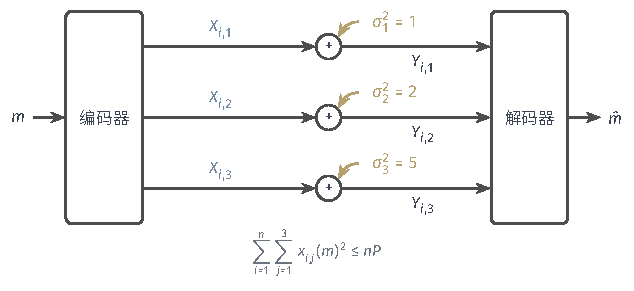
\includegraphics[width=107mm]{figures/07-probability/06-channel-coding/tikz/gcc-parallel-model/figure.pdf}
 \caption{$k=3$的平行高斯信道。第$i$次使用时，向量输入的三个分量（蓝）分别加上方差为$1,2,5$的独立噪声（黄）；三个分量和全部$n$次使用共享同一个能量预算$nP$。}
 \label{fig:gcc-parallel-model}
\end{BookInlineFigure}

\paragraph{单次使用的上界}
与标量情形一样，先在单次使用上优化。设随机输入向量$\bm{X}$的分量为$X_1,\dots,X_k$，平均能量$\mathbb{E}\lVert\bm{X}\rVert_2^2\leq P$，它与噪声向量$\bm{Z}$独立，输出$\bm{Y}=\bm{X}+\bm{Z}$。记第$j$个分量的功率为$P_j=\mathbb{E}[X_j^2]$，它们的和不超过$P$。

引理~\ref{lem:gcc-output}的证明对向量逐字成立：$\bm{Y}$有密度，$h(\bm{Y})$有限，并且
\[
 I(\bm{X};\bm{Y})=h(\bm{Y})-h(\bm{Z}) .
\]
噪声分量独立，所以$h(\bm{Z})$等于各$h(Z_j)$之和。由第~\ref{chap:information-measures}章熵的链式法则和条件化不增加熵，联合微分熵不超过各分量微分熵之和：
\[
 h(\bm{Y})\leq\sum_{j=1}^{k}h(Y_j) .
\]
每个分量的方差不超过$P_j+\sigma_j^2$，对每个分量用引理~\ref{lem:gcc-max-entropy}，得到
\begin{equation}
 I(\bm{X};\bm{Y})\leq\sum_{j=1}^{k}\bigl(h(Y_j)-h(Z_j)\bigr)\leq\sum_{j=1}^{k}\frac12\log_2\Bigl(1+\frac{P_j}{\sigma_j^2}\Bigr) .
 \label{eq:gcc-parallel-upper}
\end{equation}

这个上界可以取到：让各分量独立，$X_j\sim\mathcal{N}(0,P_j)$。此时各$Y_j$独立，次可加性取等号；每个$Y_j$是方差$P_j+\sigma_j^2$的高斯变量，熵上界也取等号。于是单次使用的问题化为一个只关于功率分配$(P_1,\dots,P_k)$的有限维问题。

\subsection{注水分配}
\label{sec:gcc-waterfilling}

要求解的是
\begin{equation}
 \max_{P_1,\dots,P_k}\ \sum_{j=1}^{k}\frac12\log_2\Bigl(1+\frac{P_j}{\sigma_j^2}\Bigr)
 \quad\text{s.t.}\quad P_j\geq0,\quad\sum_{j=1}^{k}P_j\leq P .
 \label{eq:gcc-allocation}
\end{equation}

\paragraph{边际收益}
先看每个分量多分一点功率能多得多少。第$j$项对$P_j$的导数是
\[
 \frac{\partial}{\partial P_j}\,\frac12\log_2\Bigl(1+\frac{P_j}{\sigma_j^2}\Bigr)=\frac{1}{2\ln2}\cdot\frac{1}{\sigma_j^2+P_j} .
\]
它随$P_j$增大而减小，并且在$P_j=0$处等于$1/(2\ln2\,\sigma_j^2)$：噪声越小的分量，第一份功率越值钱。于是分配应当从最安静的分量开始；它的边际收益随投入下降，降到与次安静分量的起始值相等时，再同时投入两者，使两者的边际收益保持相等，依此类推。最优时，所有分到功率的分量边际收益相同，没分到功率的分量起始收益不高于这个公共值。

\paragraph{乘子条件}
把上面的直观写成严格的最优性条件。目标函数是凹函数，约束是线性的，并且$P>0$时$P_j=P/(2k)$严格满足所有不等式约束。由卷五的凸优化理论，KKT条件对最优解既必要又充分，可参考\BookChapterRef{chap:constrained-optimality}{卷五第17章“约束问题的最优性”}。引入预算约束的乘子$\mu\geq0$与非负约束的乘子$\eta_j\geq0$，KKT条件是
\[
 \frac{1}{2\ln2}\cdot\frac{1}{\sigma_j^2+P_j}=\mu-\eta_j,\qquad \eta_jP_j=0,\qquad \mu\Bigl(P-\sum_{j}P_j\Bigr)=0 .
\]

目标函数关于每个$P_j$严格递增，预算不会留有剩余，所以$\sum_jP_j=P$且$\mu>0$。记$\nu=1/(2\ln2\,\mu)$。若$P_j>0$，则$\eta_j=0$，由第一式得$\sigma_j^2+P_j=\nu$；若$P_j=0$，则$\eta_j\geq0$，由第一式得$1/\sigma_j^2\leq1/\nu$，即$\sigma_j^2\geq\nu$。两种情形合并为$P_j=\max\{\nu-\sigma_j^2,0\}$。

\begin{theorem}[注水分配]
\label{thm:gcc-waterfilling}
设$P>0$，$\sigma_j^2>0$。问题~\eqref{eq:gcc-allocation}的唯一最优解是
\begin{equation}
 P_j=(\nu-\sigma_j^2)^{+},\qquad j=1,\dots,k,
 \label{eq:gcc-waterfilling}
\end{equation}
其中$(t)^{+}=\max\{t,0\}$，水位$\nu$是方程$\sum_{j=1}^{k}(\nu-\sigma_j^2)^{+}=P$的唯一解。平行高斯信道的信息容量是
\begin{equation}
 C(P)=\sum_{j=1}^{k}\frac12\log_2\Bigl(1+\frac{(\nu-\sigma_j^2)^{+}}{\sigma_j^2}\Bigr)
 =\sum_{j:\,\sigma_j^2<\nu}\frac12\log_2\frac{\nu}{\sigma_j^2} .
 \label{eq:gcc-parallel-capacity}
\end{equation}
\end{theorem}

\begin{proof}
函数$\nu\mapsto\sum_j(\nu-\sigma_j^2)^{+}$连续、不减，在$\nu\leq\min_j\sigma_j^2$时为零，在$\nu>\min_j\sigma_j^2$时严格递增且趋于无穷，所以方程有唯一解$\nu>\min_j\sigma_j^2$。由此定义的$P_j$非负、总和为$P$；取$\mu=1/(2\ln2\,\nu)$，$P_j>0$时取$\eta_j=0$，$P_j=0$时取$\eta_j=\mu-1/(2\ln2\,\sigma_j^2)\geq0$，KKT条件全部满足，所以它是最优解。目标函数是各分量严格凹函数之和，因而在可行集上严格凹，最优解唯一。代入目标函数，活跃分量上$1+P_j/\sigma_j^2=\nu/\sigma_j^2$，即得式~\eqref{eq:gcc-parallel-capacity}。
\end{proof}

式~\eqref{eq:gcc-waterfilling}称为\term{注水}（water-filling）分配。把第$j$个分量画成底部高度为$\sigma_j^2$的一格容器，往这排容器里倒总量为$P$的水，水面在各格中齐平，高度就是$\nu$；每格的水深就是分给它的功率。底部高于水面的格子一滴水也没有。类比的对应是：底部高度对应噪声方差，水的总量对应预算，水面齐平对应边际收益相等。类比只描述分配规则，水深与容量的关系仍要回到对数公式。

\paragraph{例：三条线路}
回到本节开头的问题：$\sigma^2=(1,2,5)$，$P=5$。把噪声方差从小到大排列，先假设只有最安静的$a$个分量活跃，由$\sum_{j\leq a}(\nu-\sigma_j^2)=P$解出
\[
 \nu_a=\frac{1}{a}\Bigl(P+\sum_{j=1}^{a}\sigma_j^2\Bigr),
\]
再检查它是否高于第$a$个、不高于第$a+1$个噪声方差。$a=3$时$\nu_3=(5+8)/3=4.33$，低于$\sigma_3^2=5$，第三个分量分不到功率，假设不成立。$a=2$时$\nu_2=(5+3)/2=4$，高于$\sigma_2^2=2$，不高于$\sigma_3^2=5$，成立。于是
\[
 \nu=4,\qquad P_1=3,\quad P_2=2,\quad P_3=0 .
\]
代入式~\eqref{eq:gcc-parallel-capacity}，容量是
\[
 C=\frac12\log_2\frac41+\frac12\log_2\frac42=1+\frac12=1.5\ \text{比特每次向量使用}.
\]

作为对照，平均分配$P_j=5/3$得到
\[
 \frac12\log_2\Bigl(1+\frac53\Bigr)+\frac12\log_2\Bigl(1+\frac56\Bigr)+\frac12\log_2\Bigl(1+\frac13\Bigr)=1.352 ;
\]
全部给第一个分量得到$\frac12\log_2 6=1.292$。平均分配把三分之一的预算放在噪声最大的分量上，那里每单位功率换来的信息最少；全部给第一个分量则让它的边际收益降到$1/(2\ln2\cdot6)$，低于第二个分量起始的$1/(2\ln2\cdot2)$。图~\ref{fig:gcc-waterfilling}(a)画出注水的结果。

\begin{BookInlineFigure}
 \centering
 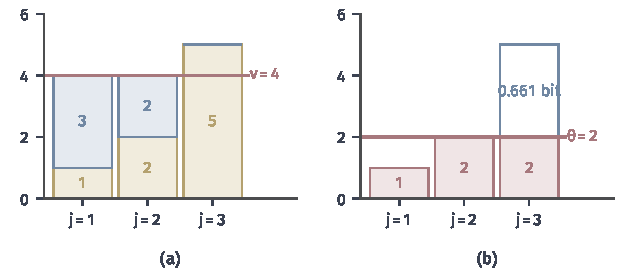
\includegraphics[width=106mm]{figures/07-probability/06-channel-coding/matplotlib/gcc-waterfilling/figure.pdf}
 \caption{两种“注水”的对照，三个分量的方差都是$(1,2,5)$。(a)平行高斯信道的功率分配，总功率$5$：黄色是噪声方差构成的底，蓝色是分到的功率，红线是水位$\nu=4$，功率为$(3,2,0)$。(b)第~\ref{chap:rate-distortion}章独立高斯分量的反注水，总失真$5$：红色是各分量的失真$\min\{\theta,\sigma_j^2\}$，红线是$\theta=2$，蓝框中高出$\theta$的部分需要描述，码率为$(0,0,0.661)$比特。}
 \label{fig:gcc-waterfilling}
\end{BookInlineFigure}

\paragraph{预算增加时}
水位随预算连续上升，分量按噪声从小到大依次加入。例中水位到达$2$时第二个分量开始分到功率，此时$P=\nu-1=1$；水位到达$5$时第三个分量加入，此时$P=(5-1)+(5-2)=7$。所以
\[
 P\leq1:\ \text{只用分量}1;\qquad 1<P\leq7:\ \text{用分量}1,2;\qquad P>7:\ \text{三个都用}.
\]
在每一段内，活跃分量的功率随$P$线性增长，斜率都是$1/a$，$a$是活跃分量数。图~\ref{fig:gcc-waterfill-path}(a)画出三条分配曲线，(b)比较三种分配方式的容量。

\begin{BookInlineFigure}
 \centering
 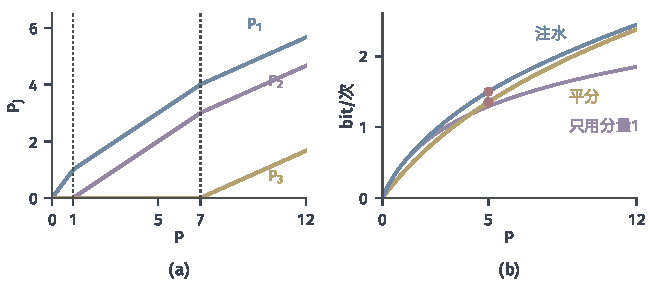
\includegraphics[width=110mm]{figures/07-probability/06-channel-coding/matplotlib/gcc-waterfill-path/figure.pdf}
 \caption{噪声方差为$(1,2,5)$时随总功率$P$的变化。(a)注水分配给三个分量的功率$P_1$（蓝）、$P_2$（紫）、$P_3$（黄），点线标出分量加入的位置$P=1$与$P=7$。(b)容量：注水分配（蓝）、平均分配（黄）、全部给分量$1$（紫）；红点是$P=5$时的$1.5$与$1.352$。}
 \label{fig:gcc-waterfill-path}
\end{BookInlineFigure}

乘子还有一层含义。由第~\ref{chap:discrete-channel-capacity}章成本约束下乘子的解释，$\mu$是预算的边际价值：总预算增加一个小量$\delta$，容量约增加$\mu\delta$。例中$\nu=4$，
\[
 \mu=\frac{1}{2\ln2\cdot4}=0.180\ \text{比特每单位功率}.
\]
直接验证：新增的功率平均分给两个活跃分量，每个水深增加$\delta/2$，每个分量的边际收益都是$1/(2\ln2\cdot4)$，容量增加约
\[
 2\cdot\frac{1}{2\ln2\cdot4}\cdot\frac{\delta}{2}=\mu\delta .
\]
第三个分量的起始边际收益是$1/(2\ln2\cdot5)=0.144$，低于$\mu=0.180$，这正是KKT条件中$\eta_3=\mu-0.144\geq0$的含义：把功率挪一点给它，只会得不偿失。

\paragraph{与反注水的对照}
第~\ref{chap:rate-distortion}章为独立高斯信源分配码率时也出现了一个“水位”，称为反注水：各分量的失真取$D_j=\min\{\theta,\sigma_j^2\}$，方差不超过$\theta$的分量不必描述。两种分配形式相似，分配的对象和方向却相反。图~\ref{fig:gcc-waterfilling}把它们并排画出，表~\ref{tab:gcc-water-vs-reverse}列出对应关系。

\begin{BookInlineTable}
 \centering
 \caption{注水与反注水的对照}
 \label{tab:gcc-water-vs-reverse}
 \begin{tabular}{lll}
  \toprule
   & 注水（信道） & 反注水（信源） \\
  \midrule
  分配的量 & 发送功率$P_j$ & 允许的失真$D_j$ \\
  分配规则 & $P_j=(\nu-\sigma_j^2)^{+}$ & $D_j=\min\{\theta,\sigma_j^2\}$ \\
  $\sigma_j^2$的含义 & 噪声方差 & 信源方差 \\
  被舍弃的分量 & 噪声高于水位 & 方差低于水位 \\
  目标 & 最大化容量 & 最小化码率 \\
  \bottomrule
 \end{tabular}
\end{BookInlineTable}

信道一侧，水倒在噪声上面，噪声越小的分量越先得到功率，因为同样的功率在那里换来更多的可区分性。信源一侧，水位以下是允许的失真，方差越大的分量越需要码率，方差小于水位的分量直接用均值重构即可。两种问题都把总资源按边际收益相等的原则分配，只是一个分配的是用来传送的资源，一个分配的是允许损失的量。

\subsection{并行传输的计量}
\label{sec:gcc-parallel-accounting}

式~\eqref{eq:gcc-parallel-capacity}是单次向量使用上的信息容量。它的单位、它与标量公式的关系，以及它是否也是块码的速率极限，需要分别说明。

\paragraph{一次向量使用}
一次使用同时占用$k$个实分量，容量计的是这$k$个分量合起来送出的比特数。例中$C=1.5$比特每次向量使用，折合每个实分量$0.5$比特；这两个数不能与单个实分量的公式~\eqref{eq:gcc-capacity}直接比较。比如把全部功率$5$放在一条噪声方差为$1$的标量信道上，得到$\frac12\log_2 6=1.292$比特每次使用，它比$1.5$小，比$0.5$大：前者比的是同一预算下“一条线路”与“三条线路”的总量，后者把三条线路的总量摊到了每条线路上。比较时要先说清楚：资源是什么（总功率还是每条线路的功率），计量单位是什么（每次向量使用还是每个实分量）。

复值信道就是$k=2$且两分量噪声相同的平行信道。两个噪声方差都是$\sigma^2/2$，注水的水位是$\nu=\sigma^2/2+P/2$，两分量平分功率，容量是
\[
 2\cdot\frac12\log_2\frac{\sigma^2/2+P/2}{\sigma^2/2}=\log_2\Bigl(1+\frac{P}{\sigma^2}\Bigr)\ \text{比特每次复值使用},
\]
这回答了第~\ref{sec:gcc-optimal-input}小节留下的问题：平分不是约定，而是最优分配。

\paragraph{可达性}
单次使用的容量能否被块码达到，回答与标量情形相同。

\begin{theorem}[平行信道的编码定理]
\label{thm:gcc-parallel-coding}
设分量数$k$固定，$P>0$，信道由式~\eqref{eq:gcc-parallel}给出，码满足约束~\eqref{eq:gcc-parallel-power}。低于式~\eqref{eq:gcc-parallel-capacity}中$C(P)$的速率都可达，且最大错误概率可以趋于零；平均错误概率趋于零的码列，其码率的上极限不超过$C(P)$。
\end{theorem}

可达性可以直接由标量结果拼出来。设$R<C(P)$，$(P_1,\dots,P_k)$是注水分配，活跃分量的集合记作$J$。因为$R<\sum_{j\in J}\frac12\log_2(1+P_j/\sigma_j^2)$，可以把$R$拆成$R=\sum_{j\in J}R_j$，使每个$R_j$严格小于第$j$个分量的标量容量。对每个$j\in J$，由定理~\ref{thm:gcc-coding}，存在第$j$个分量上满足功率约束$P_j$、码率至少$R_j$、最大错误概率$\lambda^{(j)}_{\max}\to0$的码；不活跃的分量始终发送零。

把各分量的消息组成向量$m=(m_j)_{j\in J}$，消息总数是各分量消息数之积，至少为$2^{nR}$。每条组合码字的总能量不超过$n\sum_jP_j=nP$。接收端在每个分量上独立解码，只要有一个分量判错，整条消息就判错；由并集界，最大错误概率不超过$\sum_{j\in J}\lambda^{(j)}_{\max}\to0$。

也可以不拆分，把第~\ref{sec:gcc-coding}小节的证明中的“字母”换成$k$维向量：码字在每个时刻独立地抽取$\mathcal{N}(0,P_j')$的各分量，信息密度是各分量信息密度之和，三类错误的估计逐字成立，只是能量和信息密度的平均对时刻和分量同时进行。这种做法说明向量信息密度的集中同样可以控制整组分量的联合判决。

\paragraph{逆定理}
逆向的论证与标量情形相同，只多一层对分量的求和。记$P_{i,j}=\frac1M\sum_mx_{i,j}(m)^2$为第$i$个时刻第$j$个分量在消息上的平均功率。Fano不等式和数据处理之后，与第~\ref{sec:gcc-coding}小节的第二步相同，得到
\[
 I(X^n;Y^n)\leq\sum_{i=1}^{n}F(P_{i,1},\dots,P_{i,k}),\qquad
 F(p_1,\dots,p_k)=\sum_{j=1}^{k}\frac12\log_2\Bigl(1+\frac{p_j}{\sigma_j^2}\Bigr) .
\]
$F$是凹函数，由Jensen不等式，$\sum_iF(\bm{p}_i)\leq nF(\bar{\bm{p}})$，其中$\bar{\bm{p}}$是各时刻分配向量的平均。约束~\eqref{eq:gcc-parallel-power}保证$\bar{\bm{p}}$的分量之和不超过$P$，所以$F(\bar{\bm{p}})\leq C(P)$。其余步骤与式~\eqref{eq:gcc-converse}相同。

论证依赖两个条件：分量数$k$固定，不随块长增长；噪声在时间上独立，且各分量的方差不随时刻改变。若$k$随$n$增长，或者噪声方差随时刻变化，就需要重新处理这里的大数律和单次上界。


\section{相关高斯噪声}
\label{sec:gcc-correlated}

平行信道假设各分量的噪声互相独立。两条并排的线路常常受到同一个干扰源的影响，噪声会相关。设两条线路的噪声方差都是$2$，协方差是$1$，即
\[
 \bm{Z}\sim\mathcal{N}(\bm{0},\bm{\Sigma}),\qquad \bm{\Sigma}=\begin{bmatrix}2&1\\1&2\end{bmatrix},
\]
总功率预算为$P=2$。这时各分量不能单独处理，注水规则还能用吗？功率应当分给哪个方向？

\paragraph{模型}
设$\bm{\Sigma}$是$k\times k$实对称正定矩阵。每次使用时输入$\bm{x}_i\in\mathbb{R}^k$，输出
\begin{equation}
 \bm{Y}_i=\bm{x}_i+\bm{Z}_i,\qquad \bm{Z}_1,\dots,\bm{Z}_n\ \text{独立同分布},\ \bm{Z}_i\sim\mathcal{N}(\bm{0},\bm{\Sigma}),
 \label{eq:gcc-correlated}
\end{equation}
噪声与消息独立。码字满足欧氏总能量约束$\sum_{i=1}^{n}\lVert\bm{x}_i(m)\rVert_2^2\leq nP$。同一时刻各分量的噪声可以相关，不同时刻之间仍然独立。

\paragraph{正交变换}
由谱分解（\BookChapterRef{chap:eigen-spectral-decomposition}{卷二第6章“谱分解”}），$\bm{\Sigma}=\bm{U}\bm{\Lambda}\bm{U}^{\top}$，其中$\bm{U}$是正交矩阵，列向量$\bm{u}_1,\dots,\bm{u}_k$是$\bm{\Sigma}$的单位特征向量，$\bm{\Lambda}$是以特征值$\lambda_1,\dots,\lambda_k$为对角元的对角阵，正定性保证每个$\lambda_j>0$。在特征向量的坐标下看噪声：
\[
 \tilde{\bm{Z}}=\bm{U}^{\top}\bm{Z}\sim\mathcal{N}\bigl(\bm{0},\bm{U}^{\top}\bm{\Sigma}\bm{U}\bigr)=\mathcal{N}(\bm{0},\bm{\Lambda}) .
\]
$\tilde{\bm{Z}}$的协方差矩阵是对角阵，各分量不相关；它们又是联合高斯的，由第~\ref{chap:multivariate-distributions}章，不相关的联合高斯分量相互独立。所以在这组坐标下，噪声变成了方差为$\lambda_1,\dots,\lambda_k$的独立分量。

同一组坐标也保持功率预算：$\bm{U}$是正交矩阵，对任意$\bm{x}\in\mathbb{R}^k$，
\[
 \lVert\bm{U}^{\top}\bm{x}\rVert_2=\lVert\bm{x}\rVert_2 .
\]
噪声变得独立、预算形式不变，这两点合起来说明相关噪声信道与平行信道等价。

\begin{lemma}[正交坐标下的等价]
\label{lem:gcc-rotation}
对式~\eqref{eq:gcc-correlated}的信道，记噪声方差为$\lambda_1,\dots,\lambda_k$的平行信道为$\tilde{\mathcal{C}}$。满足功率约束$P$的$(M,n)$码在两个信道之间可以一一对应，对应的码满足同样的约束，并且每条消息的条件错误概率相同。
\end{lemma}

\begin{proof}
设$(\tilde{f},\tilde{g})$是$\tilde{\mathcal{C}}$上的码，消息$m$的码字由$n$个向量$\tilde{\bm{x}}_i(m)$组成，$i=1,\dots,n$。在相关噪声信道上，令编码器发送$\bm{x}_i(m)=\bm{U}\tilde{\bm{x}}_i(m)$，解码器先把每个输出向量乘以$\bm{U}^{\top}$，再用$\tilde{g}$判决。能量逐时刻保持，所以约束成立。发送消息$m$时，
\[
 \bm{U}^{\top}\bm{Y}_i=\tilde{\bm{x}}_i(m)+\bm{U}^{\top}\bm{Z}_i ,
\]
$\bm{U}^{\top}\bm{Z}_1,\dots,\bm{U}^{\top}\bm{Z}_n$独立同分布于$\mathcal{N}(\bm{0},\bm{\Lambda})$，所以$\tilde{g}$看到的输入与在$\tilde{\mathcal{C}}$上看到的分布完全相同，条件错误概率相同。反方向把$\bm{U}$与$\bm{U}^{\top}$对调即可。
\end{proof}

图~\ref{fig:gcc-rotation-equivalence}画出这个对应：发送端和接收端各乘一个正交矩阵，中间的相关噪声信道在外面看来就是平行信道。

\begin{BookInlineFigure}
 \centering
 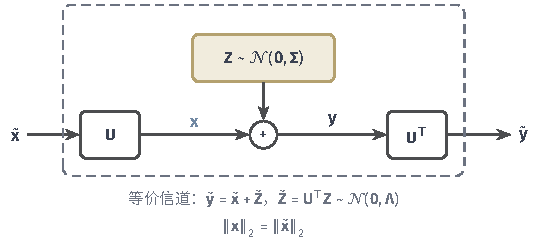
\includegraphics[width=90mm]{figures/07-probability/06-channel-coding/tikz/gcc-rotation-equivalence/figure.pdf}
 \caption{相关噪声信道与平行信道的等价。发送端把$\tilde{\bm{x}}$变成$\bm{x}=\bm{U}\tilde{\bm{x}}$，信道加上噪声$\bm{Z}\sim\mathcal{N}(\bm{0},\bm{\Sigma})$（黄框），接收端乘以$\bm{U}^{\top}$。虚线框整体是噪声方差为$\lambda_1,\dots,\lambda_k$的平行信道，正交变换保持欧氏长度。}
 \label{fig:gcc-rotation-equivalence}
\end{BookInlineFigure}

由引理~\ref{lem:gcc-rotation}和定理~\ref{thm:gcc-parallel-coding}，相关噪声信道的容量就是对特征值$\lambda_1,\dots,\lambda_k$注水得到的值。最优输入也可以写回原坐标。

\begin{theorem}[相关高斯噪声信道的容量]
\label{thm:gcc-correlated}
设$\bm{\Sigma}$正定，特征分解为$\bm{U}\bm{\Lambda}\bm{U}^{\top}$，$P>0$。式~\eqref{eq:gcc-correlated}的信道在功率约束$P$下的容量是
\begin{equation}
 C(P)=\sum_{j=1}^{k}\frac12\log_2\Bigl(1+\frac{(\nu-\lambda_j)^{+}}{\lambda_j}\Bigr),\qquad \sum_{j=1}^{k}(\nu-\lambda_j)^{+}=P .
 \label{eq:gcc-correlated-capacity}
\end{equation}
单次使用的最优输入是$\bm{X}\sim\mathcal{N}(\bm{0},\bm{K}^{\star})$，其中
\begin{equation}
 \bm{K}^{\star}=\bm{U}\operatorname{diag}\bigl((\nu-\lambda_1)^{+},\dots,(\nu-\lambda_k)^{+}\bigr)\bm{U}^{\top} ,
 \label{eq:gcc-optimal-covariance}
\end{equation}
并且
\begin{equation}
 C(P)=\max_{\bm{K}\succeq\bm{0},\ \operatorname{tr}\bm{K}\leq P}\ \frac12\log_2\frac{\det(\bm{\Sigma}+\bm{K})}{\det\bm{\Sigma}} .
 \label{eq:gcc-logdet}
\end{equation}
\end{theorem}

\begin{proof}
式~\eqref{eq:gcc-correlated-capacity}由引理~\ref{lem:gcc-rotation}与定理~\ref{thm:gcc-parallel-coding}、定理~\ref{thm:gcc-waterfilling}得到。再看式~\eqref{eq:gcc-logdet}。$k$维高斯向量$\mathcal{N}(\bm{0},\bm{A})$的微分熵是$\frac12\log_2\bigl((2\pi\mathrm{e})^k\det\bm{A}\bigr)$。对输入$\bm{X}\sim\mathcal{N}(\bm{0},\bm{K})$，输出$\bm{Y}\sim\mathcal{N}(\bm{0},\bm{\Sigma}+\bm{K})$，由$I(\bm{X};\bm{Y})=h(\bm{Y})-h(\bm{Z})$，
\[
 I(\bm{X};\bm{Y})=\frac12\log_2\frac{\det(\bm{\Sigma}+\bm{K})}{\det\bm{\Sigma}} .
\]
输入的平均能量是协方差矩阵的迹，可行的$\bm{K}$满足$\operatorname{tr}\bm{K}\leq P$。互信息在两端的可逆线性变换下不变（第~\ref{chap:information-measures}章），所以
\[
 I(\bm{X};\bm{Y})=I(\bm{U}^{\top}\bm{X};\bm{U}^{\top}\bm{Y}) ,
\]
右端是平行信道$\tilde{\mathcal{C}}$上一个满足预算的输入的互信息，由式~\eqref{eq:gcc-parallel-upper}和定理~\ref{thm:gcc-waterfilling}不超过$C(P)$。另一方面，$\bm{K}=\bm{K}^{\star}$对应平行信道上的独立高斯注水输入，取到$C(P)$。
\end{proof}

\paragraph{例：两条相关的线路}
回到本节开头的例子。$\bm{\Sigma}$的特征值和单位特征向量是
\[
 \lambda_1=1,\ \bm{u}_1=\tfrac{1}{\sqrt2}(1,-1)^{\top};\qquad \lambda_2=3,\ \bm{u}_2=\tfrac{1}{\sqrt2}(1,1)^{\top} .
\]
沿$\bm{u}_2$方向，两条线路的噪声同向，叠加得大；沿$\bm{u}_1$方向，共同的干扰在两条线路的差中抵消，只剩方差$1$。

对$(\lambda_1,\lambda_2)=(1,3)$注水，预算$P=2$。先试两个分量都活跃：$\nu=(2+1+3)/2=3$，恰好等于$\lambda_2$，第二个分量的功率是$0$。所以
\[
 \nu=3,\qquad P_1=2,\quad P_2=0,\qquad C=\frac12\log_2 3=0.792\ \text{比特每次使用}.
\]
最优输入是$\bm{X}=X_1\bm{u}_1$，$X_1\sim\mathcal{N}(0,2)$：两条线路发送大小相同、符号相反的信号，每条线路的平均功率是$1$。接收端看两条线路的差，共同干扰被抵消。

对照两种做法。若忽略相关性，让两条线路独立地各用功率$1$，即$\bm{K}=\bm{I}$，由式~\eqref{eq:gcc-logdet}，
\[
 \frac12\log_2\frac{\det(\bm{\Sigma}+\bm{I})}{\det\bm{\Sigma}}=\frac12\log_2\frac{8}{3}=0.708 .
\]
若两条线路的噪声方差仍是$2$，但相互独立，平均分配功率得到$2\cdot\frac12\log_2(1+\frac12)=0.585$。同样的边缘方差，相关的噪声反而让容量更大：相关性造出了一个噪声较小的方向，前提是发送端知道这个方向并把功率放在那里。图~\ref{fig:gcc-correlated-noise}画出原坐标和旋转后的坐标。

\begin{BookInlineFigure}
 \centering
 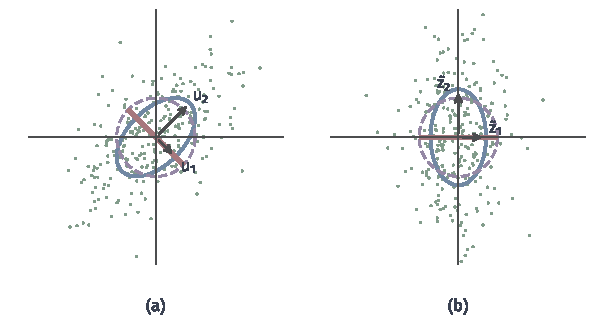
\includegraphics[width=104mm]{figures/07-probability/06-channel-coding/matplotlib/gcc-correlated-noise/figure.pdf}
 \caption{协方差为$\bm{\Sigma}=\bigl[\begin{smallmatrix}2&1\\1&2\end{smallmatrix}\bigr]$的噪声。绿点是$250$个噪声样本（种子$3$），蓝色椭圆是$\bm{z}^{\top}\bm{\Sigma}^{-1}\bm{z}=1$，黑色箭头是$\sqrt{\lambda_j}\bm{u}_j$，紫色虚线圆的半径是$\sqrt{P}=\sqrt2$，红色线段是最优输入沿$\bm{u}_1$方向的$\pm$一个标准差。(a)原坐标。(b)乘以$\bm{U}^{\top}$后的坐标，噪声分量独立，方差为$1$与$3$。}
 \label{fig:gcc-correlated-noise}
\end{BookInlineFigure}

\paragraph{白化}
另一种常见的处理是先把噪声变成单位协方差。接收端把输出乘以对称矩阵$\bm{\Sigma}^{-1/2}$，它与$\bm{\Sigma}$有相同的特征向量，特征值为$\lambda_j^{-1/2}$。这一操作称为白化：
\[
 \bar{\bm{Y}}=\bm{\Sigma}^{-1/2}\bm{Y}=\bm{\Sigma}^{-1/2}\bm{X}+\bm{N},\qquad \bm{N}=\bm{\Sigma}^{-1/2}\bm{Z}\sim\mathcal{N}(\bm{0},\bm{I}) .
\]
接收端的可逆变换可以随时撤销，不改变容量。但白化以后，信道的“输入”变成了$\bar{\bm{X}}=\bm{\Sigma}^{-1/2}\bm{X}$。若把$\bar{\bm{X}}$当作新的输入，信道是$\bar{\bm{Y}}=\bar{\bm{X}}+\bm{N}$，噪声是白的，预算却要跟着变：
\[
 \lVert\bm{X}\rVert_2^2=\lVert\bm{\Sigma}^{1/2}\bar{\bm{X}}\rVert_2^2=\bar{\bm{X}}^{\top}\bm{\Sigma}\bar{\bm{X}} .
\]
于是约束成为带权的预算
\begin{equation}
 \sum_{i=1}^{n}\bar{\bm{x}}_i^{\top}\bm{\Sigma}\bar{\bm{x}}_i\leq nP .
 \label{eq:gcc-weighted-budget}
\end{equation}
沿$\bm{u}_j$方向，$\bar{\bm{x}}$每单位平方长度要花$\lambda_j$单位的实际功率。

若忽略这一点，把白化后的问题当作单位噪声、欧氏预算的普通平行信道，注水会把功率平分，得到错误的答案。例中两个分量噪声都是$1$，平分预算$2$，得到
\[
 2\cdot\frac12\log_2(1+1)=1\ \text{比特},
\]
高于真正的容量$0.792$。多出来的部分来自一个不存在的便宜方向：沿$\bm{u}_2$放置的$\bar{\bm{x}}$实际要付三倍的功率。图~\ref{fig:gcc-whitening}画出白化后的坐标：噪声云变圆，真正的预算是紫色椭圆，错误的预算是黄色虚线圆。

\begin{BookInlineFigure}
 \centering
 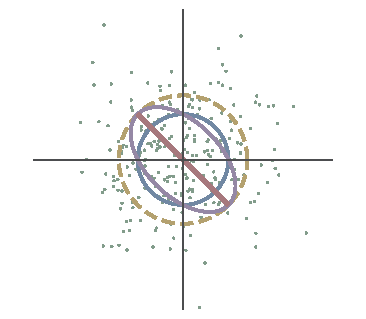
\includegraphics[width=62mm]{figures/07-probability/06-channel-coding/matplotlib/gcc-whitening/figure.pdf}
 \caption{白化后的坐标（与图~\ref{fig:gcc-correlated-noise}同一组噪声样本，绿点）。蓝圆是单位噪声的等高线；紫色椭圆是真正的预算$\bar{\bm{x}}^{\top}\bm{\Sigma}\bar{\bm{x}}\leq P$，沿$\bm{u}_1$的半轴为$\sqrt2$，沿$\bm{u}_2$的半轴为$\sqrt{2/3}$；黄色虚线圆是错误的预算$\lVert\bar{\bm{x}}\rVert_2^2\leq P$。红色线段是最优输入方向。}
 \label{fig:gcc-whitening}
\end{BookInlineFigure}

正确的做法有两种，结果相同。其一，保留原来的输入$\bm{X}$，把白化后的信道写成带增益的形式$\bar{\bm{Y}}=\bm{G}\bm{X}+\bm{N}$，$\bm{G}=\bm{\Sigma}^{-1/2}$。在特征向量坐标下，第$j$个分量是
\[
 \tilde{Y}_j=\lambda_j^{-1/2}\tilde{X}_j+N_j ,
\]
增益为$\lambda_j^{-1/2}$。两边乘以$\lambda_j^{1/2}$，得到$\tilde{X}_j$加上方差$\lambda_j$的噪声，回到对$\lambda_j$注水。其二，保留带权预算，把沿$\bm{u}_j$方向的白化输入功率记为$\bar{p}_j$，它的实际成本是$\lambda_j\bar{p}_j$，容量贡献是$\frac12\log_2(1+\bar{p}_j)$；令$P_j=\lambda_j\bar{p}_j$，问题又变成$\sum_j\frac12\log_2(1+P_j/\lambda_j)$在$\sum_jP_j\leq P$下的最大化。

\paragraph{一般的可逆变换}
上面的现象对任何可逆变换都成立。接收端的可逆变换不改变互信息，也不改变容量。发送端若用可逆矩阵$\bm{A}$换元，$\bm{X}=\bm{A}\bar{\bm{X}}$，预算中的$\lVert\bm{X}\rVert_2^2$就变成以$\bm{A}^{\top}\bm{A}$为矩阵的二次型；只有$\bm{A}$是正交矩阵时，$\bm{A}^{\top}\bm{A}=\bm{I}$，欧氏预算才保持原样。容量是“信道加约束”这一整体的性质，变换信道时必须同时变换约束。

同样的办法处理带增益矩阵的信道$\bm{Y}=\bm{H}\bm{X}+\bm{N}$，$\bm{H}$可逆，$\bm{N}\sim\mathcal{N}(\bm{0},\bm{I})$。由奇异值分解$\bm{H}=\bm{V}\bm{S}\bm{U}^{\top}$，发送端用$\bm{U}$、接收端用$\bm{V}^{\top}$，两者都是正交矩阵，信道化为增益为奇异值$s_j$的平行分量；每个分量除以增益后，等价于噪声方差为$1/s_j^2$的平行信道，再对$1/s_j^2$注水。

\paragraph{正定的作用}
定理要求$\bm{\Sigma}$正定。若$\bm{\Sigma}$有一个特征值为零，相应方向上没有噪声：沿这个方向发送任意实数，接收端在这个方向上的投影就是它本身，于是不同的实数都能被区分，容量为无穷。特征值很小但为正时，容量有限；这个方向的水底最低，注水时它最先分到功率。


\section{本章小结}
\label{sec:gcc-summary}

本章回答了章首的问题：独立高斯噪声下，每次使用在功率预算$P$内最多能可靠送出多少比特。答案由三层论证组成。

第一层是上界。输入二阶矩有限、噪声独立且方差为正时，输出有密度，互信息等于输出熵减去噪声熵；输出方差不超过$P+\sigma^2$，固定方差时高斯分布的熵最大，于是单次互信息不超过$\frac12\log_2(1+P/\sigma^2)$。去掉任何一个条件，结论都可能失效：不限功率或噪声方差为零时，容量没有上限。

第二层把上界连接到可靠传输。零均值高斯输入$\mathcal{N}(0,P)$使输出仍为高斯并达到上界，它是唯一的最优输入。坐标独立服从$\mathcal{N}(0,P')$、$P'<P$的随机码配合信息密度的阈值判决，使发送的码字以接近一的概率越过门限、其他码字以指数小的概率越过门限；超预算和错误偏高的码字在删去一半消息时一并去掉，得到满足逐条功率约束、最大错误趋于零的码。反方向由Fano不等式、逐时刻的熵上界和容量对功率的凹性给出。两者合起来，$C_{\mathrm{op}}(P)=\frac12\log_2(1+P/\sigma^2)$比特每次实值使用，单位换成复值使用或每秒时须一起换算功率和使用次数。

第三层处理多个分量。独立的平行分量把单次问题化为功率分配，最优分配是注水：低噪声分量先得到功率，所有活跃分量的边际收益相等，噪声高于水位的分量不用。它与率失真中的反注水形式相似，但分配的是发送功率而不是允许的失真。相关噪声经正交变换变成独立分量，欧氏预算保持不变，容量是对噪声协方差的特征值注水；白化同样可用，但必须把预算一起变换成带权的形式。

\begin{BookInlineTable}
 \centering
 \caption{本章的三种高斯信道}
 \label{tab:gcc-summary}
 \begin{tabular}{llll}
  \toprule
  模型 & 噪声 & 容量 & 最优输入 \\
  \midrule
  标量 & $\mathcal{N}(0,\sigma^2)$ & $\frac12\log_2(1+P/\sigma^2)$ & $\mathcal{N}(0,P)$ \\
  平行 & 独立，方差$\sigma_j^2$ & 对$\sigma_j^2$注水 & 独立，功率$(\nu-\sigma_j^2)^{+}$ \\
  相关 & $\mathcal{N}(\bm{0},\bm{\Sigma})$ & 对特征值$\lambda_j$注水 & $\mathcal{N}(\bm{0},\bm{K}^{\star})$ \\
  \bottomrule
 \end{tabular}
\end{BookInlineTable}

这些结论都依赖指定的条件：噪声与输入独立，各次使用之间独立，噪声方差或协方差固定并为发送端所知，分量数固定，预算按每条码字计算。噪声在时间上相关、信道带有记忆或反馈时，需要随机过程的工具重新建立单次上界与大数律，可参考\BookChapterRef{chap:discrete-time-stochastic-processes}{卷九第3章“离散时间随机过程”}。容量定理是关于块长趋于无穷的陈述：图~\ref{fig:gcc-random-code}已经显示，有限块长下距离容量还有明显的差距，随机码本的存储和最近码字的搜索也随块长指数增长。下一章转向可以实际构造和译码的有限长度纠错码。

